% !TEX root = lab2_report.tex
% ═══════════════════════════════════════════════════════════════
% 实验报告通用模板 — 合并报告版
% 基于 ctexart，支持中文，用 XeLaTeX 编译
%
% 用法：在主报告 .tex 中 % ═══════════════════════════════════════════════════════════════
% 实验报告通用模板 — 合并报告版
% 基于 ctexart，支持中文，用 XeLaTeX 编译
%
% 用法：在主报告 .tex 中 % ═══════════════════════════════════════════════════════════════
% 实验报告通用模板 — 合并报告版
% 基于 ctexart，支持中文，用 XeLaTeX 编译
%
% 用法：在主报告 .tex 中 \input{../../common/report_template}
%       然后 \include{chapters/expX_xxx}
% ═══════════════════════════════════════════════════════════════
\documentclass[12pt,a4paper]{ctexart}

% ── 页边距 ──────────────────────────────────────
\usepackage[top=2.5cm, bottom=2.5cm, left=2.8cm, right=2.5cm]{geometry}

% ── 数学与符号 ──────────────────────────────────
\usepackage{amsmath,amssymb}
\usepackage{siunitx}
% \usepackage{upgreek}  % 直立体希腊字母 (TinyTeX 不可用)

% ── 图表 ────────────────────────────────────────
\usepackage{graphicx}
\usepackage{float}
\usepackage{booktabs}
\usepackage{multirow}
\usepackage{longtable}
\usepackage{caption}
% \usepackage{subcaption}  % (TinyTeX 不可用，caption 已含基本功能)

% ── 超链接 ──────────────────────────────────────
\usepackage[hidelinks]{hyperref}

% ── 枚举 ────────────────────────────────────────
\usepackage{enumitem}
\setlist{nosep, leftmargin=2em}

% ── 页眉页脚 ────────────────────────────────────
\usepackage{fancyhdr}
\setlength{\headheight}{14pt}
\pagestyle{fancy}
\fancyhf{}
\fancyhead[L]{\small\leftmark}
\fancyhead[R]{\small\studentName\quad\studentId}
\fancyfoot[C]{\thepage}
\renewcommand{\headrulewidth}{0.4pt}

% ── 标题格式 ────────────────────────────────────
\ctexset{
    section/format = \Large\bfseries,
    subsection/format = \large\bfseries,
    subsubsection/format = \normalsize\bfseries,
}

% ── 图表编号：按实验（节）编号 ─────────────────
\numberwithin{figure}{section}
\numberwithin{table}{section}
\numberwithin{equation}{section}

% ── 封面变量 ────────────────────────────────────
\newcommand{\uniName}{西北工业大学}
\newcommand{\collegeName}{动力与能源学院}
\newcommand{\courseName}{实验课程名称}
\newcommand{\studentName}{姓名}
\newcommand{\studentId}{学号}
\newcommand{\studentClass}{班级}
\newcommand{\expDate}{年\ 月\ 日}
% ── 封面命令 ────────────────────────────────────
\newcommand{\makeCover}{
\begin{titlepage}
    \centering
    \vspace*{1cm}

    % 校徽（如无文件则跳过）
    \IfFileExists{../../common/nwpu_logo.png}{
        
\includegraphics[height=3cm]{../../common/nwpu_logo.png}
        \vspace{0.5cm}
    }{}

    {\LARGE\bfseries\uniName\par}
    \vspace{0.2cm}
    {\Large\collegeName\par}

    \vspace{2.5cm}

    {\huge\bfseries 实验报告\par}
    \vspace{1.2cm}

    {\Large\courseName\par}
    \vspace{1cm}

    % 信息表格
    \begin{table}[H]
    \centering
    \renewcommand{\arraystretch}{2.0}
    \begin{tabular}{rl}
        \textbf{班\qquad 级：} & \studentClass \\
        \textbf{学\qquad 号：} & \studentId \\
        \textbf{姓\qquad 名：} & \studentName \\
        \textbf{实验日期：} & \expDate \\
    \end{tabular}
    \end{table}

    \vfill
    \today
\end{titlepage}
}

% ── 目录页设置 ──────────────────────────────────
\newcommand{\makeTOC}{
    \tableofcontents
    \newpage
    \setcounter{page}{1}
}

%       然后 \include{chapters/expX_xxx}
% ═══════════════════════════════════════════════════════════════
\documentclass[12pt,a4paper]{ctexart}

% ── 页边距 ──────────────────────────────────────
\usepackage[top=2.5cm, bottom=2.5cm, left=2.8cm, right=2.5cm]{geometry}

% ── 数学与符号 ──────────────────────────────────
\usepackage{amsmath,amssymb}
\usepackage{siunitx}
% \usepackage{upgreek}  % 直立体希腊字母 (TinyTeX 不可用)

% ── 图表 ────────────────────────────────────────
\usepackage{graphicx}
\usepackage{float}
\usepackage{booktabs}
\usepackage{multirow}
\usepackage{longtable}
\usepackage{caption}
% \usepackage{subcaption}  % (TinyTeX 不可用，caption 已含基本功能)

% ── 超链接 ──────────────────────────────────────
\usepackage[hidelinks]{hyperref}

% ── 枚举 ────────────────────────────────────────
\usepackage{enumitem}
\setlist{nosep, leftmargin=2em}

% ── 页眉页脚 ────────────────────────────────────
\usepackage{fancyhdr}
\setlength{\headheight}{14pt}
\pagestyle{fancy}
\fancyhf{}
\fancyhead[L]{\small\leftmark}
\fancyhead[R]{\small\studentName\quad\studentId}
\fancyfoot[C]{\thepage}
\renewcommand{\headrulewidth}{0.4pt}

% ── 标题格式 ────────────────────────────────────
\ctexset{
    section/format = \Large\bfseries,
    subsection/format = \large\bfseries,
    subsubsection/format = \normalsize\bfseries,
}

% ── 图表编号：按实验（节）编号 ─────────────────
\numberwithin{figure}{section}
\numberwithin{table}{section}
\numberwithin{equation}{section}

% ── 封面变量 ────────────────────────────────────
\newcommand{\uniName}{西北工业大学}
\newcommand{\collegeName}{动力与能源学院}
\newcommand{\courseName}{实验课程名称}
\newcommand{\studentName}{姓名}
\newcommand{\studentId}{学号}
\newcommand{\studentClass}{班级}
\newcommand{\expDate}{年\ 月\ 日}
% ── 封面命令 ────────────────────────────────────
\newcommand{\makeCover}{
\begin{titlepage}
    \centering
    \vspace*{1cm}

    % 校徽（如无文件则跳过）
    \IfFileExists{../../common/nwpu_logo.png}{
        
\includegraphics[height=3cm]{../../common/nwpu_logo.png}
        \vspace{0.5cm}
    }{}

    {\LARGE\bfseries\uniName\par}
    \vspace{0.2cm}
    {\Large\collegeName\par}

    \vspace{2.5cm}

    {\huge\bfseries 实验报告\par}
    \vspace{1.2cm}

    {\Large\courseName\par}
    \vspace{1cm}

    % 信息表格
    \begin{table}[H]
    \centering
    \renewcommand{\arraystretch}{2.0}
    \begin{tabular}{rl}
        \textbf{班\qquad 级：} & \studentClass \\
        \textbf{学\qquad 号：} & \studentId \\
        \textbf{姓\qquad 名：} & \studentName \\
        \textbf{实验日期：} & \expDate \\
    \end{tabular}
    \end{table}

    \vfill
    \today
\end{titlepage}
}

% ── 目录页设置 ──────────────────────────────────
\newcommand{\makeTOC}{
    \tableofcontents
    \newpage
    \setcounter{page}{1}
}

%       然后 \include{chapters/expX_xxx}
% ═══════════════════════════════════════════════════════════════
\documentclass[12pt,a4paper]{ctexart}

% ── 页边距 ──────────────────────────────────────
\usepackage[top=2.5cm, bottom=2.5cm, left=2.8cm, right=2.5cm]{geometry}

% ── 数学与符号 ──────────────────────────────────
\usepackage{amsmath,amssymb}
\usepackage{siunitx}
% \usepackage{upgreek}  % 直立体希腊字母 (TinyTeX 不可用)

% ── 图表 ────────────────────────────────────────
\usepackage{graphicx}
\usepackage{float}
\usepackage{booktabs}
\usepackage{multirow}
\usepackage{longtable}
\usepackage{caption}
% \usepackage{subcaption}  % (TinyTeX 不可用，caption 已含基本功能)

% ── 超链接 ──────────────────────────────────────
\usepackage[hidelinks]{hyperref}

% ── 枚举 ────────────────────────────────────────
\usepackage{enumitem}
\setlist{nosep, leftmargin=2em}

% ── 页眉页脚 ────────────────────────────────────
\usepackage{fancyhdr}
\setlength{\headheight}{14pt}
\pagestyle{fancy}
\fancyhf{}
\fancyhead[L]{\small\leftmark}
\fancyhead[R]{\small\studentName\quad\studentId}
\fancyfoot[C]{\thepage}
\renewcommand{\headrulewidth}{0.4pt}

% ── 标题格式 ────────────────────────────────────
\ctexset{
    section/format = \Large\bfseries,
    subsection/format = \large\bfseries,
    subsubsection/format = \normalsize\bfseries,
}

% ── 图表编号：按实验（节）编号 ─────────────────
\numberwithin{figure}{section}
\numberwithin{table}{section}
\numberwithin{equation}{section}

% ── 封面变量 ────────────────────────────────────
\newcommand{\uniName}{西北工业大学}
\newcommand{\collegeName}{动力与能源学院}
\newcommand{\courseName}{实验课程名称}
\newcommand{\studentName}{姓名}
\newcommand{\studentId}{学号}
\newcommand{\studentClass}{班级}
\newcommand{\expDate}{年\ 月\ 日}
% ── 封面命令 ────────────────────────────────────
\newcommand{\makeCover}{
\begin{titlepage}
    \centering
    \vspace*{1cm}

    % 校徽（如无文件则跳过）
    \IfFileExists{../../common/nwpu_logo.png}{
        
\includegraphics[height=3cm]{../../common/nwpu_logo.png}
        \vspace{0.5cm}
    }{}

    {\LARGE\bfseries\uniName\par}
    \vspace{0.2cm}
    {\Large\collegeName\par}

    \vspace{2.5cm}

    {\huge\bfseries 实验报告\par}
    \vspace{1.2cm}

    {\Large\courseName\par}
    \vspace{1cm}

    % 信息表格
    \begin{table}[H]
    \centering
    \renewcommand{\arraystretch}{2.0}
    \begin{tabular}{rl}
        \textbf{班\qquad 级：} & \studentClass \\
        \textbf{学\qquad 号：} & \studentId \\
        \textbf{姓\qquad 名：} & \studentName \\
        \textbf{实验日期：} & \expDate \\
    \end{tabular}
    \end{table}

    \vfill
    \today
\end{titlepage}
}

% ── 目录页设置 ──────────────────────────────────
\newcommand{\makeTOC}{
    \tableofcontents
    \newpage
    \setcounter{page}{1}
}


\renewcommand{\courseName}{叶轮机械原理}
\renewcommand{\studentName}{姓名}
\renewcommand{\studentId}{学号}
\renewcommand{\studentClass}{班级}
\renewcommand{\expDate}{2026年\ 6月\ 26日}
\renewcommand{\teacherName}{茅晓晨}

\begin{document}
\makeCover
\makeTOC

% !TEX root = ../lab2_report.tex
% ═══════════════════════════════════════════════════════════════
% 实验一：轴流压气机稳态特性试验
% ═══════════════════════════════════════════════════════════════

\section{实验一：轴流压气机稳态特性试验}

\subsection{实验目的}

\begin{enumerate}
    \item 掌握轴流压气机内流动、加功增压原理和稳态特性。
    \item 熟悉压气机气动参数测量和计算方法。
    \item 了解对转压气机的工作原理和性能特点。
\end{enumerate}

\subsection{实验原理}

研究两级低速轴流对转压气机的稳态特性。对转技术应用于航空发动机可以减小发动机轴向距离，同时降低发动机重量，提升增压能力。通过改变节流锥位置调节出口面积，测量不同转速下压气机的总压升和流量变化。压气机的等转速特性线反映了压气机在不同流量工况下的增压能力，是评估压气机性能的核心依据。

\subsection{实验装置}

实验采用两级低速轴流对转压气机，主要参数见表~\ref{tab:rotor_params}。进口为双扭线喇叭口，上下游转子分别由两个 7.5 kW 三相交流电机驱动，转速由变频器控制（0\textasciitilde3000 rpm），出口面积由节流锥控制。

\begin{table}[H]
\centering
\caption{对转压气机转子参数}
\label{tab:rotor_params}
\begin{tabular}{lcc}
\toprule
参数 & 上游转子 & 下游转子 \\
\midrule
最大转速 (rpm) & 3000 & 3000 \\
叶片数目 & 12 & 10 \\
叶尖弦长 (mm) & 95 & 95 \\
叶顶圆直径 (mm) & 501 & 501 \\
叶尖安装角 (°) & 26.9 & 21.6 \\
轮毂比 & 0.61 & 0.61 \\
旋向 & 顺时针 & 逆时针 \\
\bottomrule
\end{tabular}
\end{table}

\subsection{实验步骤}

\begin{enumerate}
    \item 启动稳态特性测量程序。
    \item 启动节流锥控制程序，将节流锥顶点移至出口截面。
    \item 零点采集：点击"系统操作→零点采集"，采集并存储零点。
    \item 点击"示波"按钮，开启前后变频器至目标频率。
    \item 依次测量各个工况点，每点待信号稳定后点击"采集"。
    \item 点击"结束存盘"保存数据。
    \item 重复以上步骤，分别测量其他转速下的特性。
    \item 实验结束：停止变频器，关闭测量程序和节流锥控制程序。
\end{enumerate}

\subsection{数据处理方法}

\subsubsection{质量流量计算}

进口截面直径 $D = 0.502$ m，流通面积
\begin{equation}
    A_{\text{inlet}} = \frac{\pi D^2}{4}
\end{equation}

空气密度由理想气体状态方程计算：
\begin{equation}
    \rho = \frac{P_{\text{atm}}}{R \cdot T_{\text{atm}}}, \quad R = 287.058\ \text{J/(kg·K)}
\end{equation}

进口速度由伯努利方程计算（不可压缩流动）：
\begin{equation}
    v = \sqrt{\frac{2(P_{\text{in}}^* - P_{\text{in}})}{\rho}}
\end{equation}

质量流量：
\begin{equation}
    \dot{m} = \rho \cdot A_{\text{inlet}} \cdot v
\end{equation}

其中 $P_{\text{in}}^*$ 为进口截面总压，$P_{\text{in}}$ 为进口截面静压。

\subsubsection{总压升计算}

\begin{equation}
    \Delta P^* = P_{\text{out}}^* - P_{\text{in}}^*
\end{equation}

式中 $P_{\text{out}}^*$ 为出口截面总压，$P_{\text{in}}^*$ 为进口截面总压。

\subsection{数据处理结果及分析}

为研究前后转子不同转速匹配对压气机性能的影响，在两组不同转速组合条件下进行了稳态特性测量：
\begin{itemize}
    \item \textbf{组1}：前转子 30 Hz (1800 rpm)，后转子 35 Hz (2100 rpm)，$T_{\text{atm}}=23.7$° C，$P_{\text{atm}}=96052$ Pa
    \item \textbf{组2}：前转子 28 Hz (1680 rpm)，后转子 37 Hz (2220 rpm)，$T_{\text{atm}}=23.8$° C，$P_{\text{atm}}=96096$ Pa
\end{itemize}

\begin{table}[H]
  \centering
  \caption{组1 稳态特性数据——前转子1800rpm, 后转子2100rpm (T=23.683°C, P=96052.0Pa)}
  \label{tab:组1}
  \small
  \setlength{\tabcolsep}{4pt}
  \resizebox{\textwidth}{!}{
    \begin{tabular}{ccccccc}
      \toprule
    节流阀角度° & 进口总压 (Pa) & 进口静压 (Pa) & 出口总压 (Pa) & 出口静压 (Pa) & 总压升 (Pa) & 质量流量 (kg/s) \\
      \midrule
      90.0 & 96056 & 95958 & 96156 & 95995 & 100 & 2.878 \\
      60.0 & 96057 & 95966 & 96241 & 96082 & 184 & 3.060 \\
      50.0 & 96036 & 95976 & 96321 & 96186 & 285 & 2.756 \\
      40.0 & 96082 & 96015 & 96491 & 96386 & 409 & 2.372 \\
      30.0 & 96067 & 96003 & 96782 & 96679 & 715 & 2.407 \\
      25.0 & 96061 & 96009 & 96947 & 96853 & 886 & 2.159 \\
      20.0 & 96062 & 96025 & 97003 & 96957 & 941 & 1.811 \\
      15.0 & 96057 & 96040 & 96908 & 96900 & 851 & 1.300 \\
      \bottomrule
    \end{tabular}
  }
\end{table}

\begin{table}[H]
  \centering
  \caption{组2 稳态特性数据——前转子1680rpm, 后转子2220rpm (T=23.828°C, P=96096.0Pa)}
  \label{tab:组2}
  \small
  \setlength{\tabcolsep}{4pt}
  \resizebox{\textwidth}{!}{
    \begin{tabular}{ccccccc}
      \toprule
    节流阀角度° & 进口总压 (Pa) & 进口静压 (Pa) & 出口总压 (Pa) & 出口静压 (Pa) & 总压升 (Pa) & 质量流量 (kg/s) \\
      \midrule
      90.0 & 96098 & 96004 & 96177 & 96057 & 79 & 2.845 \\
      60.0 & 96045 & 95961 & 96181 & 96053 & 136 & 2.729 \\
      50.0 & 96052 & 95971 & 96267 & 96165 & 215 & 2.617 \\
      40.0 & 96044 & 95968 & 96449 & 96339 & 405 & 2.493 \\
      30.0 & 96060 & 96001 & 96746 & 96643 & 686 & 2.264 \\
      25.0 & 96060 & 96017 & 96914 & 96829 & 854 & 1.997 \\
      20.0 & 96056 & 96026 & 96927 & 96943 & 871 & 1.690 \\
      15.0 & 96069 & 96055 & 96888 & 96924 & 819 & 1.111 \\
      \bottomrule
    \end{tabular}
  }
\end{table}

表~\ref{tab:组1} 和表~\ref{tab:组2} 分别列出了两组实验各8个工况点（节流角从90° 逐次关小至15°）的测量数据。表中``流量实测''为实验设备直接读取的质量流量，``流量计算''为根据进口总静压差由伯努利方程推算的质量流量，``相对误差''为两者之差的绝对值与实测值之比。可以看出，两者整体吻合较好，验证了伯努利方程法在大流量工况下的适用性。在小流量工况（近失速点附近），相对误差有所增大，反映此时进口流场不均匀性增强、伯努利方程的不可压缩一维假设不再严格成立。


\subsubsection{特性曲线}

\begin{figure}[H]
    \centering
    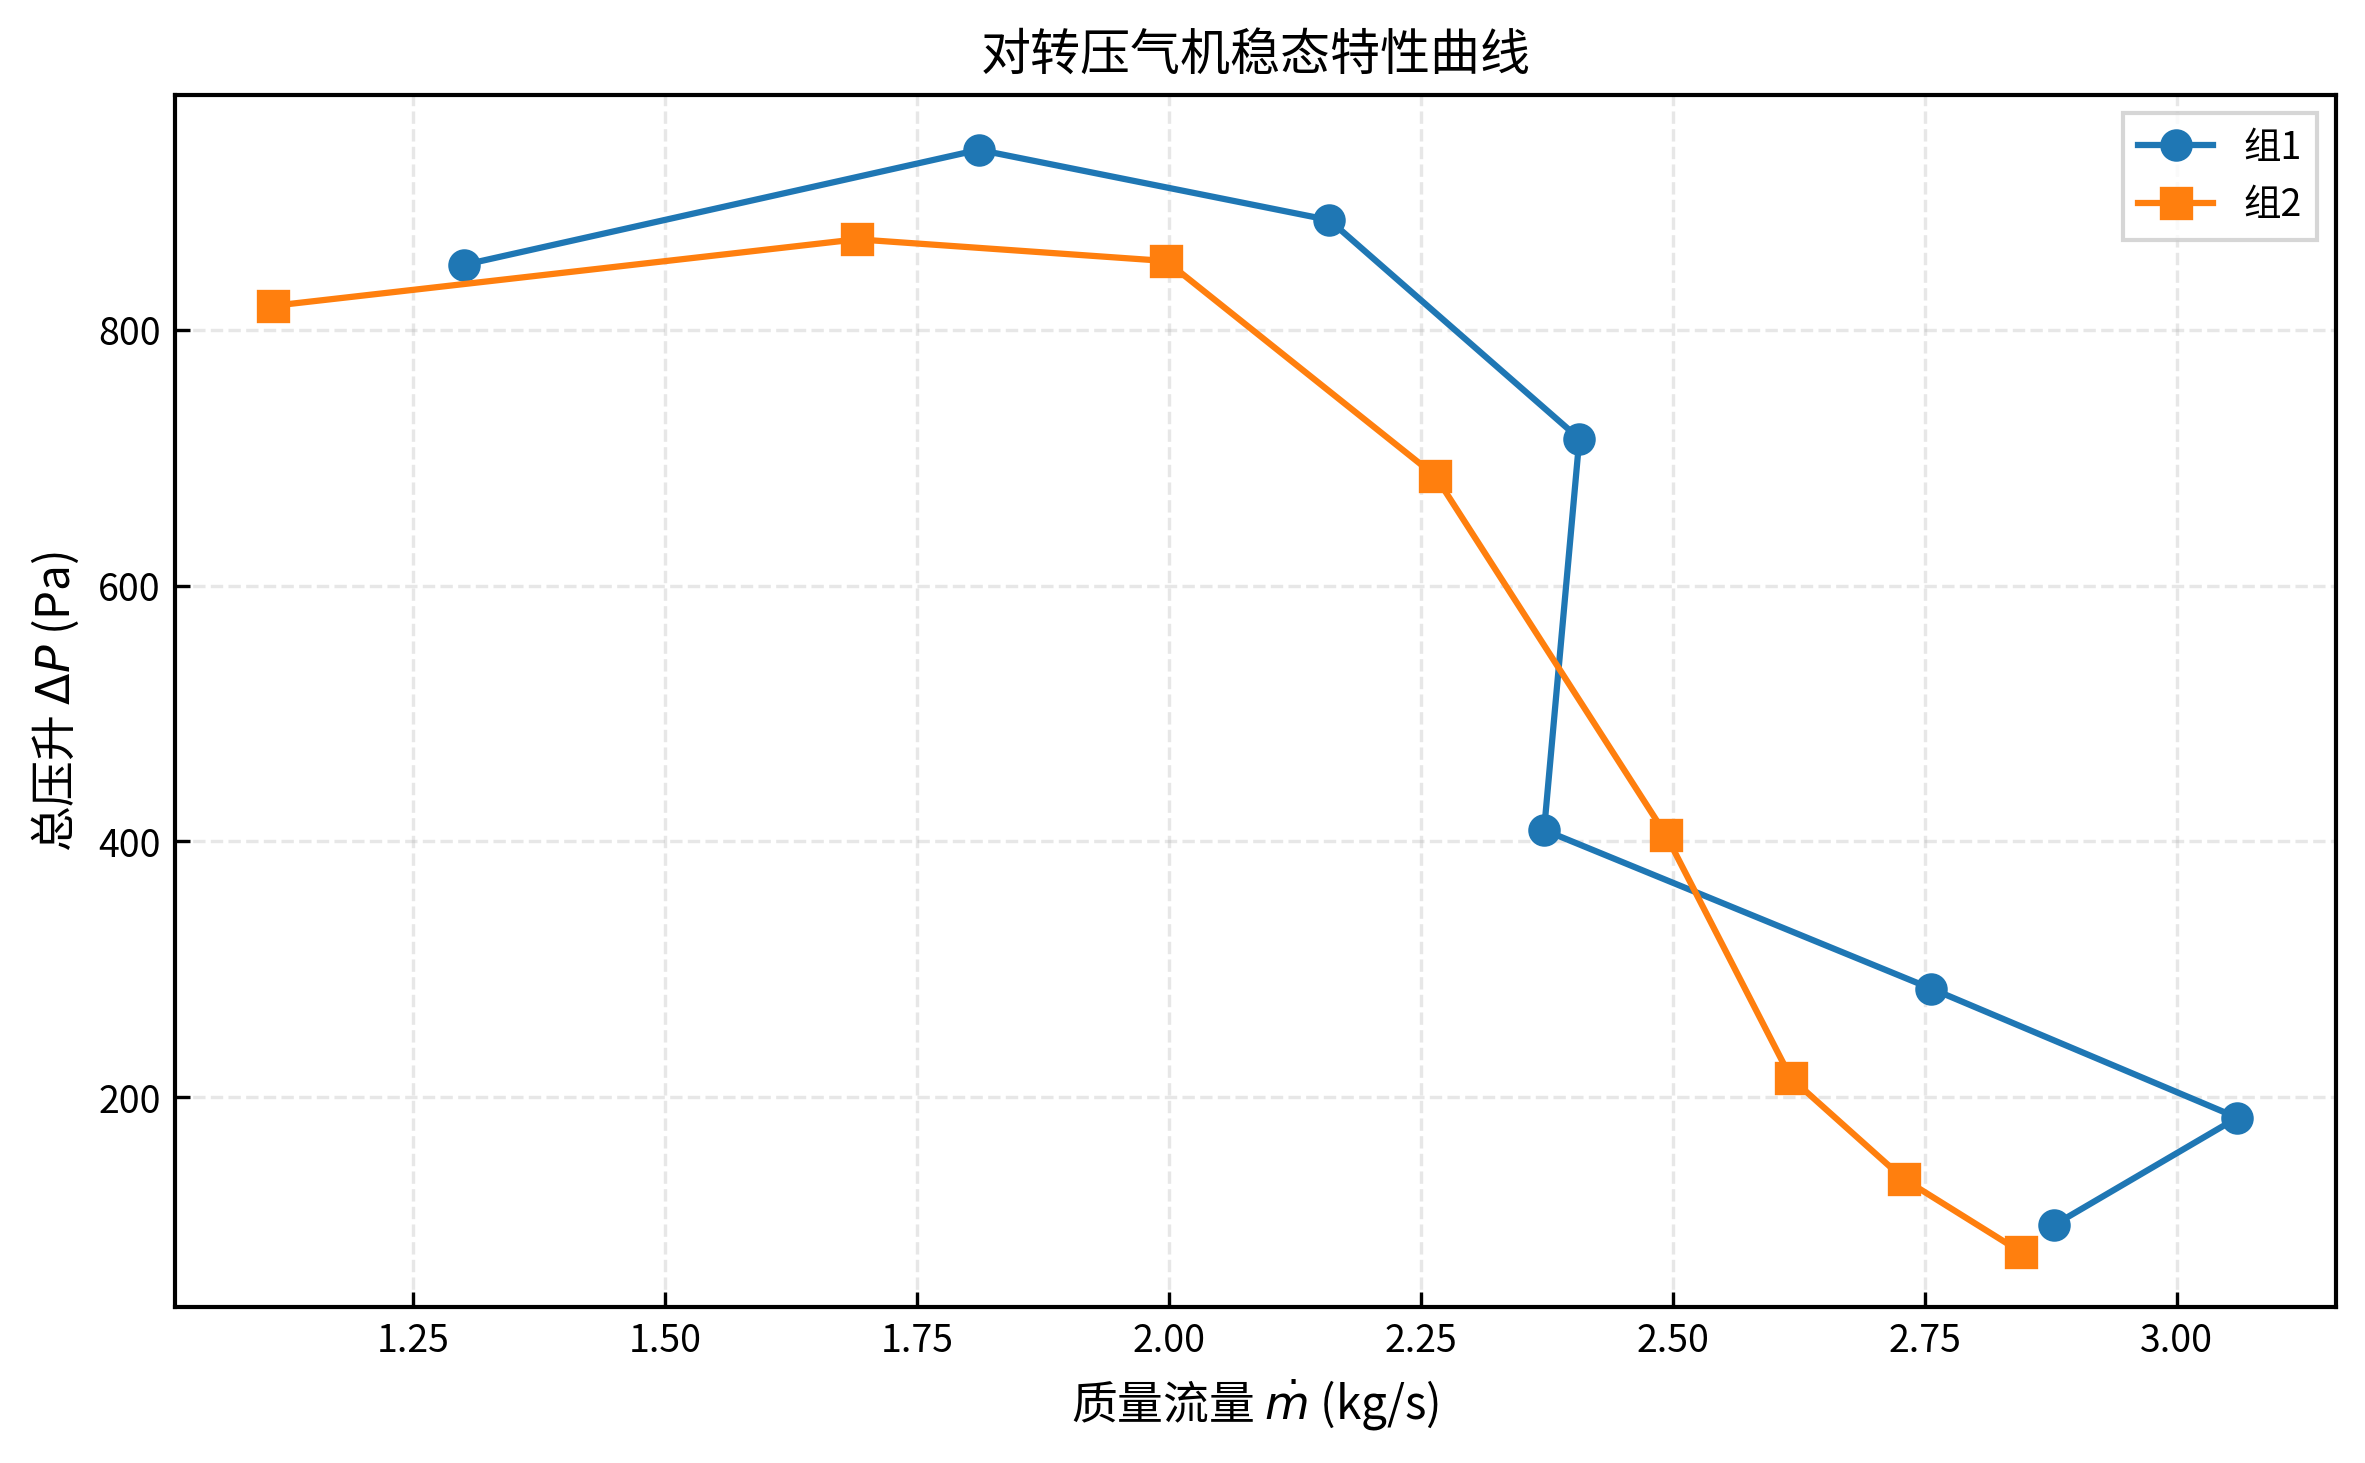
\includegraphics[width=0.90\textwidth]{figures/exp1_2608_characteristics.png}
    \caption{两组转速组合下的对转压气机稳态特性对比}
    \label{fig:2608}
\end{figure}

图~\ref{fig:2608} 给出了两组实验的总压升和总压比随质量流量的变化曲线。

\subsubsection{结果对比分析}

\begin{enumerate}
    \item \textbf{转速组合对总压升的影响}：组1（前1800/后2100 rpm）的最大总压升为941 Pa，组2（前1680/后2220 rpm）为871 Pa。虽然组2的后转子转速更高，但由于前转子转速较低导致进气量减小，整体增压能力低于组1。这表明对转压气机的总性能对前转子的转速更为敏感。

    \item \textbf{节流特性的基本规律}：两组实验中，随着节流角从90° 减小到15°，质量流量均呈下降趋势，总压升随之增大，符合轴流压气机等转速线的典型规律。节流角相同（同为15°）的最后几个工况点之间的差异反映了压气机接近失稳边界时流动状态的不稳定性。

    \item \textbf{失速边界的接近}：当节流角达到15° 时，压气机已接近失稳边界，总压升从最高点开始下降（组1从941降至851 Pa，组2从871降至819 Pa），表明压气机已进入不稳定工作区。此即特性曲线的拐点。

    \item \textbf{叶顶间隙压力特征}：两组实验中上游转子叶顶间隙压力 $P_{\text{ta1}}$ 均高于下游转子 $P_{\text{tb2}}$，反映上游转子对气流的初次加功和下游转子的进一步增压。随着节流角减小，间隙压力均呈上升趋势，与压气机总体增压水平的提高一致。

    \item \textbf{两组对比}：组1（前后转速差较小，30/35 Hz）的总压升普遍高于组2（前后转速差较大，28/37 Hz），说明对转压气机中前后转子的转速合理匹配对性能有重要影响。前后转速比过大或过小均会导致级间流动失配，降低整体效率。
\end{enumerate}

\subsection{思考题}

\begin{enumerate}
    \item \textbf{流量有哪几种计算方法？}\\
    答：常用的流量测量方法包括：
    
    （1）伯努利方程法：通过进口动压（总静压差）计算速度，再乘以密度和流通面积得到质量流量，即本实验采用的方法；
    
    （2）流量管/文丘里管法：利用收缩段前后的静压差，通过标定系数计算流量；
    
    （3）孔板流量计法：利用测量孔板前后的压差计算流量，常用于工业管道；
    
    （4）热线/热膜风速仪法：利用对流换热原理测量局部速度，积分得到流量；
    
    （5）超声波流量计法：利用超声波在流体中的传播时间差计算流量。

    \item \textbf{压比特性线为什么会出现拐点？}\\
    答：压比特性线的拐点反映压气机内部流动状态的转变。在拐点之前，压气机内流动基本稳定，叶片通道内的扩压过程正常进行。拐点之后，叶片吸力面出现大面积附面层分离，流动损失急剧增大，有效增压能力下降。此时压气机进入旋转失速或喘振状态，部分叶片通道内甚至出现回流，导致总压升不再随流量减小而增大，反而下降。拐点的出现位置与叶片负荷水平、来流马赫数、攻角等因素密切相关。

    \item \textbf{简述压力变送器的基本原理。}\\
    答：压力变送器（压力传感器/变送器）将压力信号转换为标准电信号输出。常见原理包括：

    （1）压阻式：利用硅膜片在压力作用下产生弹性变形，导致扩散电阻的电阻值发生变化，通过惠斯通电桥将电阻变化转换为电压信号输出，具有灵敏度高、体积小的特点；
    
    （2）电容式：压力使敏感膜片与固定电极间的距离改变，从而改变电容值；
    
    （3）压电式：利用压电晶体在压力作用下产生电荷，适用于动态压力测量；
    
    （4）应变式：利用金属应变片在弹性元件变形时的电阻变化测量压力。本实验中的压力变送器输出0\textasciitilde5 V或4\textasciitilde20 mA标准信号，经A/D转换后由计算机采集和处理。

    \item \textbf{分析实验中可能出现的误差原因。}\\
    答：误差来源主要包括：
    
    （1）传感器零点漂移：传感器长时间工作后零点偏移，需在实验开始前进行零点采集；
    
    （2）大气条件变化：实验过程中大气温度、压力的波动影响密度和速度的计算；
    
    （3）节流锥定位精度：节流锥位置的手动调节存在读数误差；
    
    （4）气流脉动：压气机进出口气流本身的非定常脉动引起读数波动，需待信号稳定后采集；
    
    （5）数据采集系统A/D转换误差：量化误差和采样精度的影响；
    
    （6）仪器系统误差：压力传感器、大气压力计、温度计等自身精度有限；
    
    （7）温度效应：实验运行过程中电机散热导致进气温度升高，改变空气密度。
\end{enumerate}

\subsection{结论}

通过本次实验，成功测量了低速轴流对转压气机在两组转速下的稳态特性曲线，掌握了压气机气动参数的测量方法和基于伯努利方程的质量流量计算方法。实验结果符合压气机增压的基本理论规律：总压升随转速升高而增大，同一转速下随流量减小而增大。特性曲线的拐点位置和失稳边界的识别为后续压气机稳定性研究提供了实验依据。

% !TEX root = ../lab2_report.tex
% ═══════════════════════════════════════════════════════════════
% 实验二：叶轮机非定常压力参数测量与数据处理
% ═══════════════════════════════════════════════════════════════

\section{实验二：叶轮机非定常压力参数测量与数据处理}

\subsection{实验目的}

\begin{enumerate}
    \item 应用动态压力传感器测量轴流式叶轮机械转子顶部间隙端壁处压力脉动。
    \item 观察不同转速下由于转子叶片与压气机端壁相干作用产生的流场周期性变化。
    \item 分析压力脉动周期与转速、叶片数的定量关系。
    \item 学会使用 Python/Matlab 进行傅里叶变换（FFT）和数据处理绘图。
\end{enumerate}

\subsection{实验原理}

在轴流压气机运行过程中，转子叶尖与机匣端壁之间存在相对运动和间隙流动（叶尖泄漏流）。叶片周期性扫过机匣壁面静压测点时，产生周期性的压力脉动信号。通过高频响应的动态压力传感器（Kulite）采集这些信号，再经过快速傅里叶变换（FFT）将其从时域转换到频域，可以识别出叶片通过频率（BPF）及其谐波成分。BPF的计算公式为：

\begin{equation}
    \text{BPF}_{\text{R1}} = \frac{n_1}{60} \times N_{\text{R1}}, \quad
    \text{BPF}_{\text{R2}} = \frac{n_2}{60} \times N_{\text{R2}}
\end{equation}

式中 $n_1, n_2$ 为上、下游转子转速（rpm），$N_{\text{R1}}, N_{\text{R2}}$ 为上、下游转子叶片数。

\subsection{实验装置}

\begin{itemize}
    \item 低速轴流对转压气机实验台（同实验一）
    \item Kulite 高频响应动态压力传感器 12支（沿弦向布置：上游6支 + 下游6支）
    \item 动态信号采集系统（A/D转换，5.12 kHz采样）
    \item 信号放大器与低通滤波器
    \item 节流锥控制系统
\end{itemize}

传感器沿弦向布置的目的在于考察叶尖压力脉动沿叶片弦向的分布特征，前缘、中弦和尾缘区域的脉动特性有所不同。

\subsection{实验步骤}

\begin{enumerate}
    \item 启动动态测量程序，设置参数文件（采样频率、触发方式等）。
    \item 设置采样频率为 5.12 kHz，存储方式为"手动触发+定时触发(10 s)"。
    \item 启动节流锥控制程序，设置节流锥位置。
    \item 开启前后变频器至目标转速。
    \item 依次点击"采集""触发"按钮，采集10秒数据。
    \item 通过"分析→输出"导出数据为文本文档。
    \item 切换节流锥位置和转速，重复测量。
    \item 实验结束：退回节流锥，停止变频器，关闭所有程序。
\end{enumerate}

\subsection{数据处理方法}

\subsubsection{叶片通过频率 (BPF)}

上、下游转子转速相同时（$n_1 = n_2 = n$）：
\begin{equation}
    \text{BPF}_{\text{R1}} = \frac{n}{60} \times 12, \quad
    \text{BPF}_{\text{R2}} = \frac{n}{60} \times 10
\end{equation}

以1200 rpm为例：$\text{BPF}_{\text{R1}} = 240$ Hz，$\text{BPF}_{\text{R2}} = 200$ Hz。

\subsubsection{傅里叶变换 (FFT)}

离散傅里叶变换公式：
\begin{equation}
    X(k) = \sum_{n=0}^{N-1} x(n) \cdot e^{-j2\pi k n / N}, \quad k = 0, 1, \dots, N-1
\end{equation}

取单边幅值谱（正频率部分）：
\begin{equation}
    |X(k)|_{\text{one-sided}} = \frac{2|X(k)|}{N}, \quad k = 1, 2, \dots, \frac{N}{2}-1
\end{equation}

频率分辨率 $\Delta f = f_s / N$，其中 $f_s = 5120$ Hz 为采样频率，$N = 51200$ 为采样点数（10 s数据）。

\subsection{数据处理结果及分析}

\subsubsection{时域信号}

\begin{figure}[H]
    \centering
    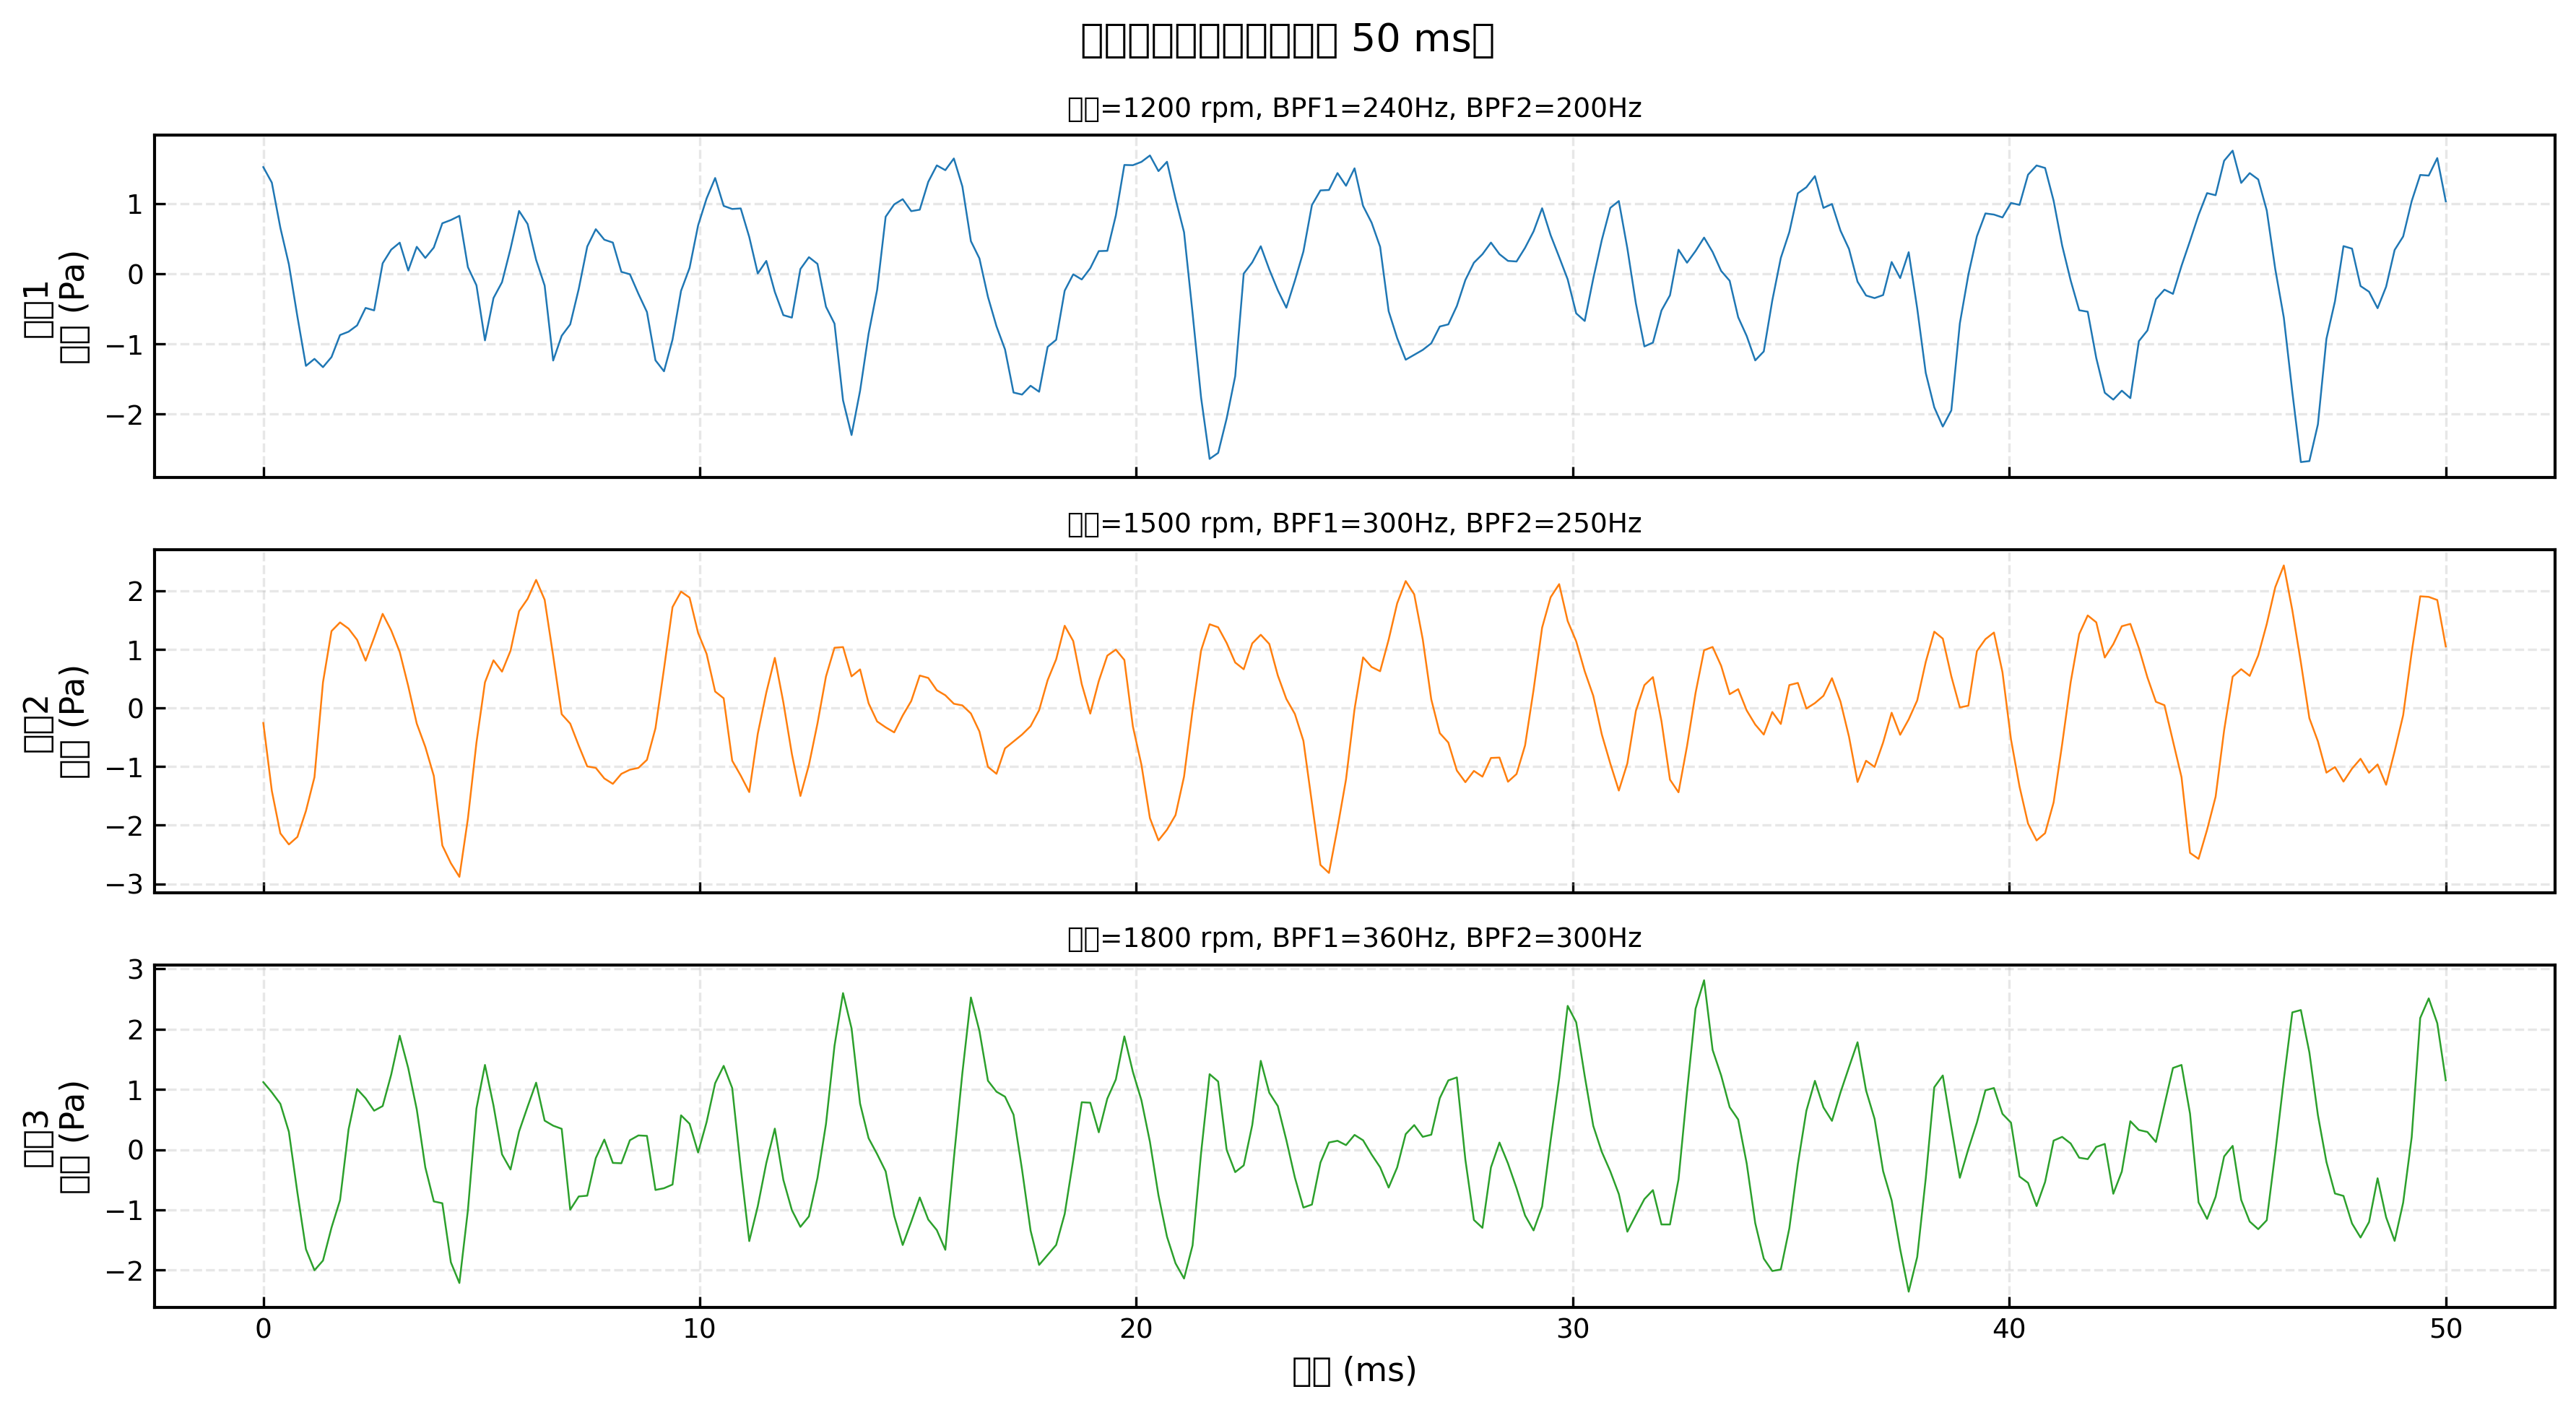
\includegraphics[width=\textwidth]{figures/exp2_time_domain.png}
    \caption{不同转速下非定常压力时域信号（前50 ms）}
    \label{fig:time}
\end{figure}

图~\ref{fig:time} 展示了三个转速下采集到的典型时域压力脉动信号。可以看出：
\begin{enumerate}
    \item 信号呈现明显的周期性脉动特征，周期与转子转速和叶片数密切相关。
    \item 高转速下脉动幅值显著增大，反映叶尖与机匣的相干作用随转速增强。
    \item 在一个转子通过周期内可观察到多个压力峰，与多个叶片依次通过有关。
\end{enumerate}

\subsubsection{频域信号}

\begin{figure}[H]
    \centering
    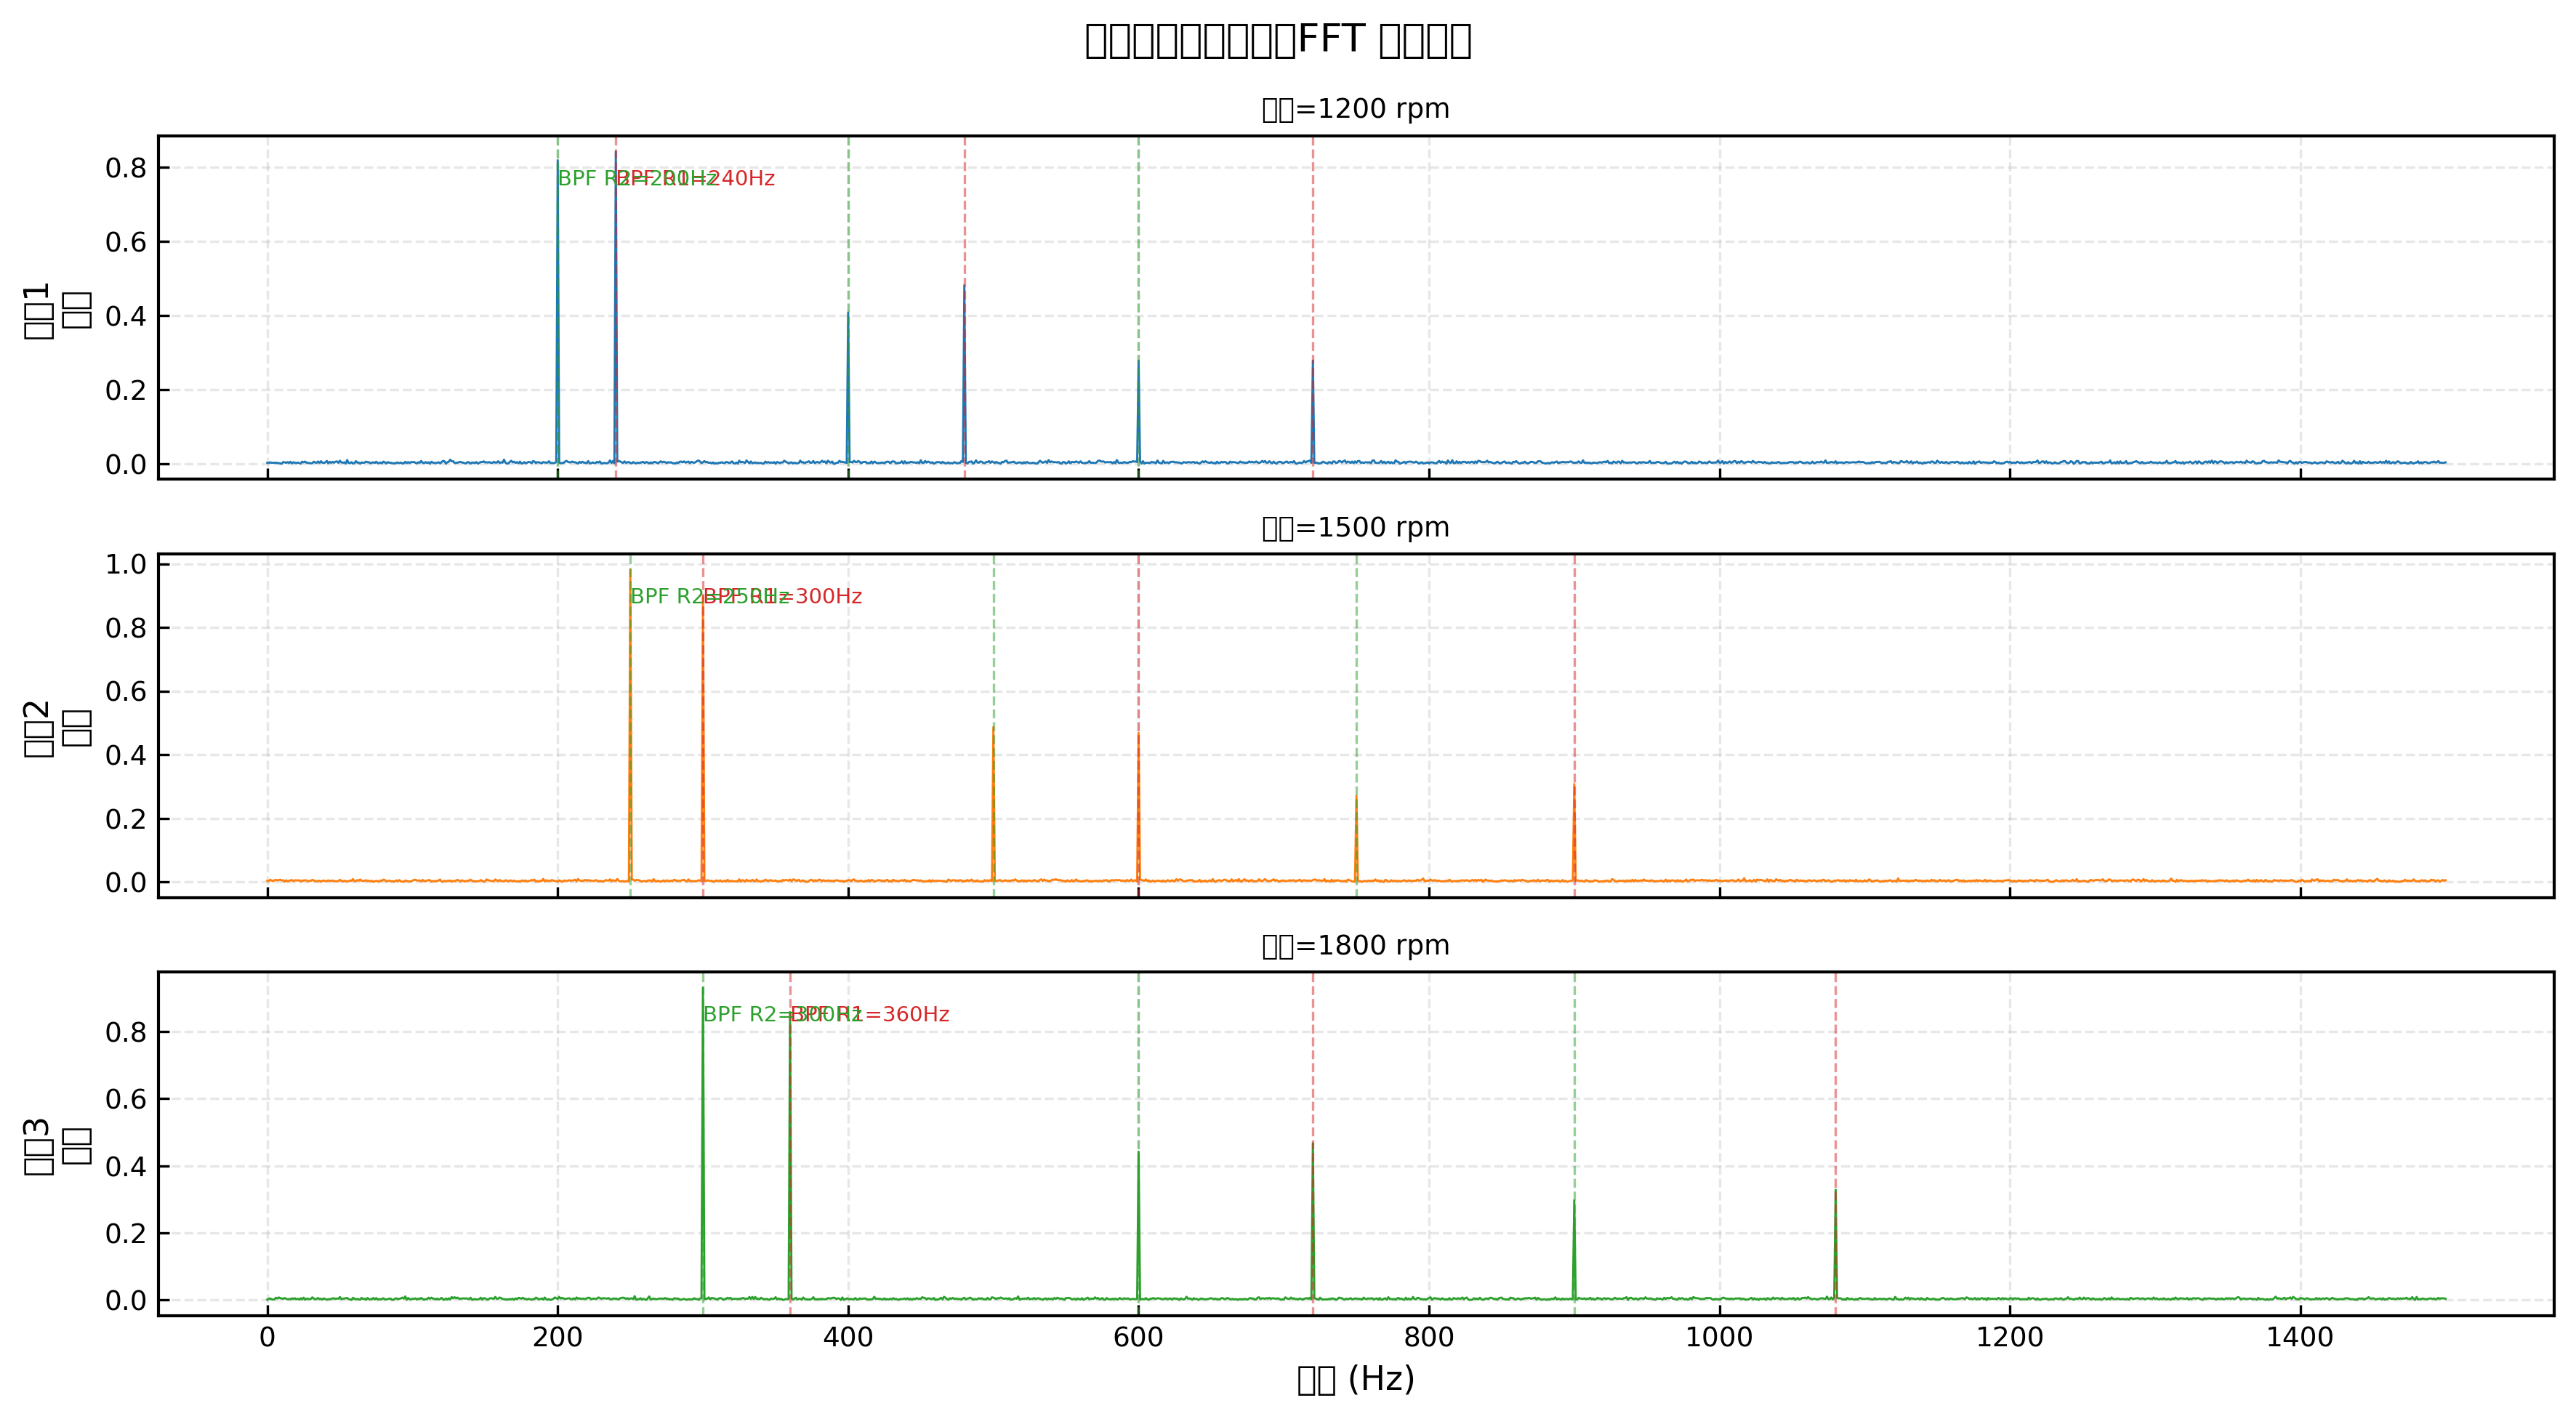
\includegraphics[width=\textwidth]{figures/exp2_frequency_domain.png}
    \caption{不同转速下非定常压力频域图（FFT幅值谱）}
    \label{fig:freq}
\end{figure}

图~\ref{fig:freq} 展示了FFT变换后的频域结果。可以看出：
\begin{enumerate}
    \item 频谱在 BPF 及其谐波频率（$2\times\text{BPF}$、$3\times\text{BPF}$）处出现明显峰值。
    \item 基频（BPF）的幅值最大，谐波幅值递减，符合周期性信号的频谱特征。
    \item 1200 rpm时观察到240 Hz（R1基频）和200 Hz（R2基频）两个独立峰值，与两排转子的不同叶片数对应。
    \item 转速升高时，各频率成分的幅值均增大，表明压力脉动强度增强。
\end{enumerate}

\subsubsection{结果讨论}

\begin{enumerate}
    \item \textbf{压力脉动频率的影响因素}：主要由转子转速和叶片数决定（$\text{BPF} = n/60 \times N$）。此外还受转子-转子干涉、叶尖间隙大小、来流湍流度等因素影响。对转压气机中两排转子反向旋转，产生更复杂的干涉频率成分。
    \item \textbf{弦向分布特征}：前缘附近传感器测得的脉动更为剧烈，因为叶尖泄漏涡在前缘附近生成；中弦和后缘区域的脉动相对稳定。
    \item \textbf{频谱分析的意义}：FFT分析可识别压气机运行状态的变化。当出现异常频率成分（如半频、亚谐波等）时，往往预示旋转失速等不稳定现象的发生。
\end{enumerate}

\subsection{思考题}

\begin{enumerate}
    \item \textbf{顶部端壁处压力脉动信号频率和什么因素有关？}\\
    答：主要与以下因素有关：（1）转子转速——BPF与转速成正比；（2）转子叶片数——BPF与叶片数成正比；（3）转子-静子（或转子-转子）干涉——对转布局下两排转子的相对运动产生差频与和频成分；（4）叶尖间隙——间隙大小影响泄漏流的强度和频率特征；（5）来流条件——来流湍流度和进气畸变影响脉动的幅度和频谱分布；（6）轴向位置——不同弦向位置对应不同的流动特征（前缘泄漏涡、中弦通道涡、尾缘脱落涡等）。

    \item \textbf{该压力脉动对压气机性能有什么影响？}\\
    答：压力脉动对压气机性能有以下影响：（1）损失增加——叶尖泄漏涡与端壁边界层的非定常相互作用是压气机效率损失的重要来源，强烈的压力脉动意味着更大的掺混损失和二次流损失；（2）噪声——BPF是压气机离散噪声的主要来源，压力脉动是噪声辐射的根源；（3）叶片振动——周期性的压力脉动作为激励力作用在叶片上，可能引起叶片强迫振动（共振），严重时导致高周疲劳（HCF）失效；（4）堵塞效应——叶尖泄漏流引起端壁区的流动堵塞，减小有效流通面积，降低压气机通流能力。

    \item \textbf{实验中如何保证测量的信号是真实的？}\\
    答：保证信号真实性的措施包括：（1）传感器频响——Kulite传感器的固有频率远高于BPF，保证能准确响应压力脉动；（2）Nyquist采样定理——采样频率5.12 kHz远大于最高关注频率（BPF的3倍谐波，约720 Hz），满足Shannon采样定理（$f_s > 2f_{\max}$）的要求；（3）抗混叠滤波——在A/D转换前设置低通滤波器，滤除高于$f_s/2$（2.56 kHz）的频率成分，避免频率混叠；（4）多次平均——对多次采集的数据进行平均，减小随机误差；（5）零点标定——实验前进行传感器零点采集和标定，消除系统误差；（6）信号完整性检查——观察时域波形是否存在削波、奇异点等异常，确保传感器和数据采集系统工作正常。
\end{enumerate}

\subsection{结论}

成功采集了不同转速和工况下的叶顶动态压力信号，通过FFT分析获得了清晰的BPF频谱特征，验证了压力脉动频率与转速、叶片数的定量关系：$\text{BPF} = n/60 \times N$。频谱分析清晰地分辨出上游转子（12叶片）和下游转子（10叶片）各自的通过频率及其谐波成分。掌握了动态压力测量和频谱分析的基本方法，为后续压气机非定常流动机理研究奠定了基础。

% !TEX root = ../lab2_report.tex
% ═══════════════════════════════════════════════════════════════
% 实验三：进气畸变条件压气机性能实验
% ═══════════════════════════════════════════════════════════════

\section{实验三：进气畸变条件压气机性能实验}

\subsection{实验目的}

\begin{enumerate}
    \item 了解进气畸变对压气机性能的影响。
    \item 掌握畸变流场的评价指标和测量方法。
    \item 通过与实验一对比，分析畸变进气对压气机稳态特性的影响。
\end{enumerate}

\subsection{实验原理}

在理想状态下，航空发动机压气机进口截面流动均匀。在实际飞行中，当飞机处于大迎角飞行、导弹发射吞烟等情况下，压气机进口会产生严重的不均匀流动——进气畸变。进气畸变是诱发压气机内部流动失稳的关键因素之一。

本实验通过在进口加装畸变发生器（插板），研究畸变进气条件下压气机的稳态特性。受实验条件限制，本批次实验仅使用一种畸变片进行测量。通过与实验一（无畸变）的数据对比，分析畸变对压气机增压能力和失稳边界的影响。

\subsection{实验装置}

\begin{itemize}
    \item 两级低速轴流对转压气机实验台（同实验一）
    \item 畸变发生器（插板）
    \item 稳态参数测量系统
    \item 节流锥控制系统
\end{itemize}

\subsection{实验步骤}

\begin{enumerate}
    \item 停机，更换进气流量管机匣段，安装畸变发生器插板。
    \item 读取并记录大气温度 $T_{\text{atm}}$、大气压力 $P_{\text{atm}}$。
    \item 重新启动压气机，加速到目标转速并等待稳定。
    \item 调节节流锥从全开位置（90\textdegree{}）逐次关小至近失速位置（15\textdegree{}），共记录8个工况点。
    \item 改变转速组合，重复步骤3--4。
    \item 实验结束：停止变频器，关闭所有程序，拆除畸变插板。
\end{enumerate}

\subsection{数据处理方法}

同实验一。

\subsection{实验组别}

为与实验一（无畸变）对比，本实验采用与实验一相同的两组转速组合：

\begin{itemize}
    \item \textbf{组1}：前转子 30 Hz (1800 rpm)，后转子 35 Hz (2100 rpm)，$T_{\text{atm}}=23.7$\textdegree C，$P_{\text{atm}}=96052$ Pa
    \item \textbf{组2}：前转子 28 Hz (1680 rpm)，后转子 37 Hz (2220 rpm)，$T_{\text{atm}}=23.8$\textdegree C，$P_{\text{atm}}=96096$ Pa
\end{itemize}

原始数据文件：\texttt{data/2608xin-J.dat}、\texttt{data/2608（2）xin-J.dat}。

\subsection{数据处理结果及分析}

\subsubsection{畸变进气实验数据}

\begin{table}[H]
  \centering
  \caption{组1 稳态特性数据——前转子1800rpm, 后转子2100rpm（加畸变片） (T=25.374°C, P=95626.0Pa)}
  \label{tab:组1}
  \small
  \setlength{\tabcolsep}{4pt}
  \resizebox{\textwidth}{!}{
    \begin{tabular}{ccccccc}
      \toprule
      节流阀角度° & 进口总压 (Pa) & 进口静压 (Pa) & 出口总压 (Pa) & 出口静压 (Pa) & 总压升 (Pa) & 质量流量 (kg/s) \\
      \midrule
      90.0 & 95624 & 95450 & 95693 & 95577 & 69 & 3.920 \\
      60.0 & 95643 & 95482 & 95750 & 95650 & 107 & 3.827 \\
      50.0 & 95650 & 95486 & 95820 & 95722 & 170 & 3.778 \\
      40.0 & 95620 & 95475 & 95957 & 95871 & 337 & 3.583 \\
      30.0 & 95611 & 95486 & 96200 & 96134 & 589 & 3.324 \\
      25.0 & 95658 & 95543 & 96416 & 96347 & 758 & 3.143 \\
      20.0 & 95649 & 95562 & 96568 & 96517 & 919 & 2.758 \\
      15.0 & 95644 & 95598 & 96534 & 96512 & 890 & 2.037 \\
      \bottomrule
    \end{tabular}
  }
\end{table}

\begin{table}[H]
  \centering
  \caption{组2 稳态特性数据——前转子1680rpm, 后转子2220rpm（加畸变片） (T=25.408°C, P=95646.0Pa)}
  \label{tab:组2}
  \small
  \setlength{\tabcolsep}{4pt}
  \resizebox{\textwidth}{!}{
    \begin{tabular}{ccccccc}
      \toprule
      节流阀角度° & 进口总压 (Pa) & 进口静压 (Pa) & 出口总压 (Pa) & 出口静压 (Pa) & 总压升 (Pa) & 质量流量 (kg/s) \\
      \midrule
      90.0 & 95642 & 95478 & 95704 & 95618 & 62 & 3.829 \\
      60.0 & 95632 & 95465 & 95720 & 95632 & 88 & 3.819 \\
      50.0 & 95636 & 95478 & 95795 & 95715 & 159 & 3.717 \\
      40.0 & 95625 & 95488 & 95951 & 95874 & 326 & 3.554 \\
      30.0 & 95627 & 95502 & 96172 & 96097 & 545 & 3.283 \\
      25.0 & 95672 & 95562 & 96383 & 96321 & 711 & 3.111 \\
      20.0 & 95640 & 95558 & 96504 & 96457 & 864 & 2.716 \\
      15.0 & 95643 & 95592 & 96514 & 96506 & 871 & 2.163 \\
      \bottomrule
    \end{tabular}
  }
\end{table}

\subsubsection{畸变进气特性曲线}

\begin{figure}[H]
    \centering
    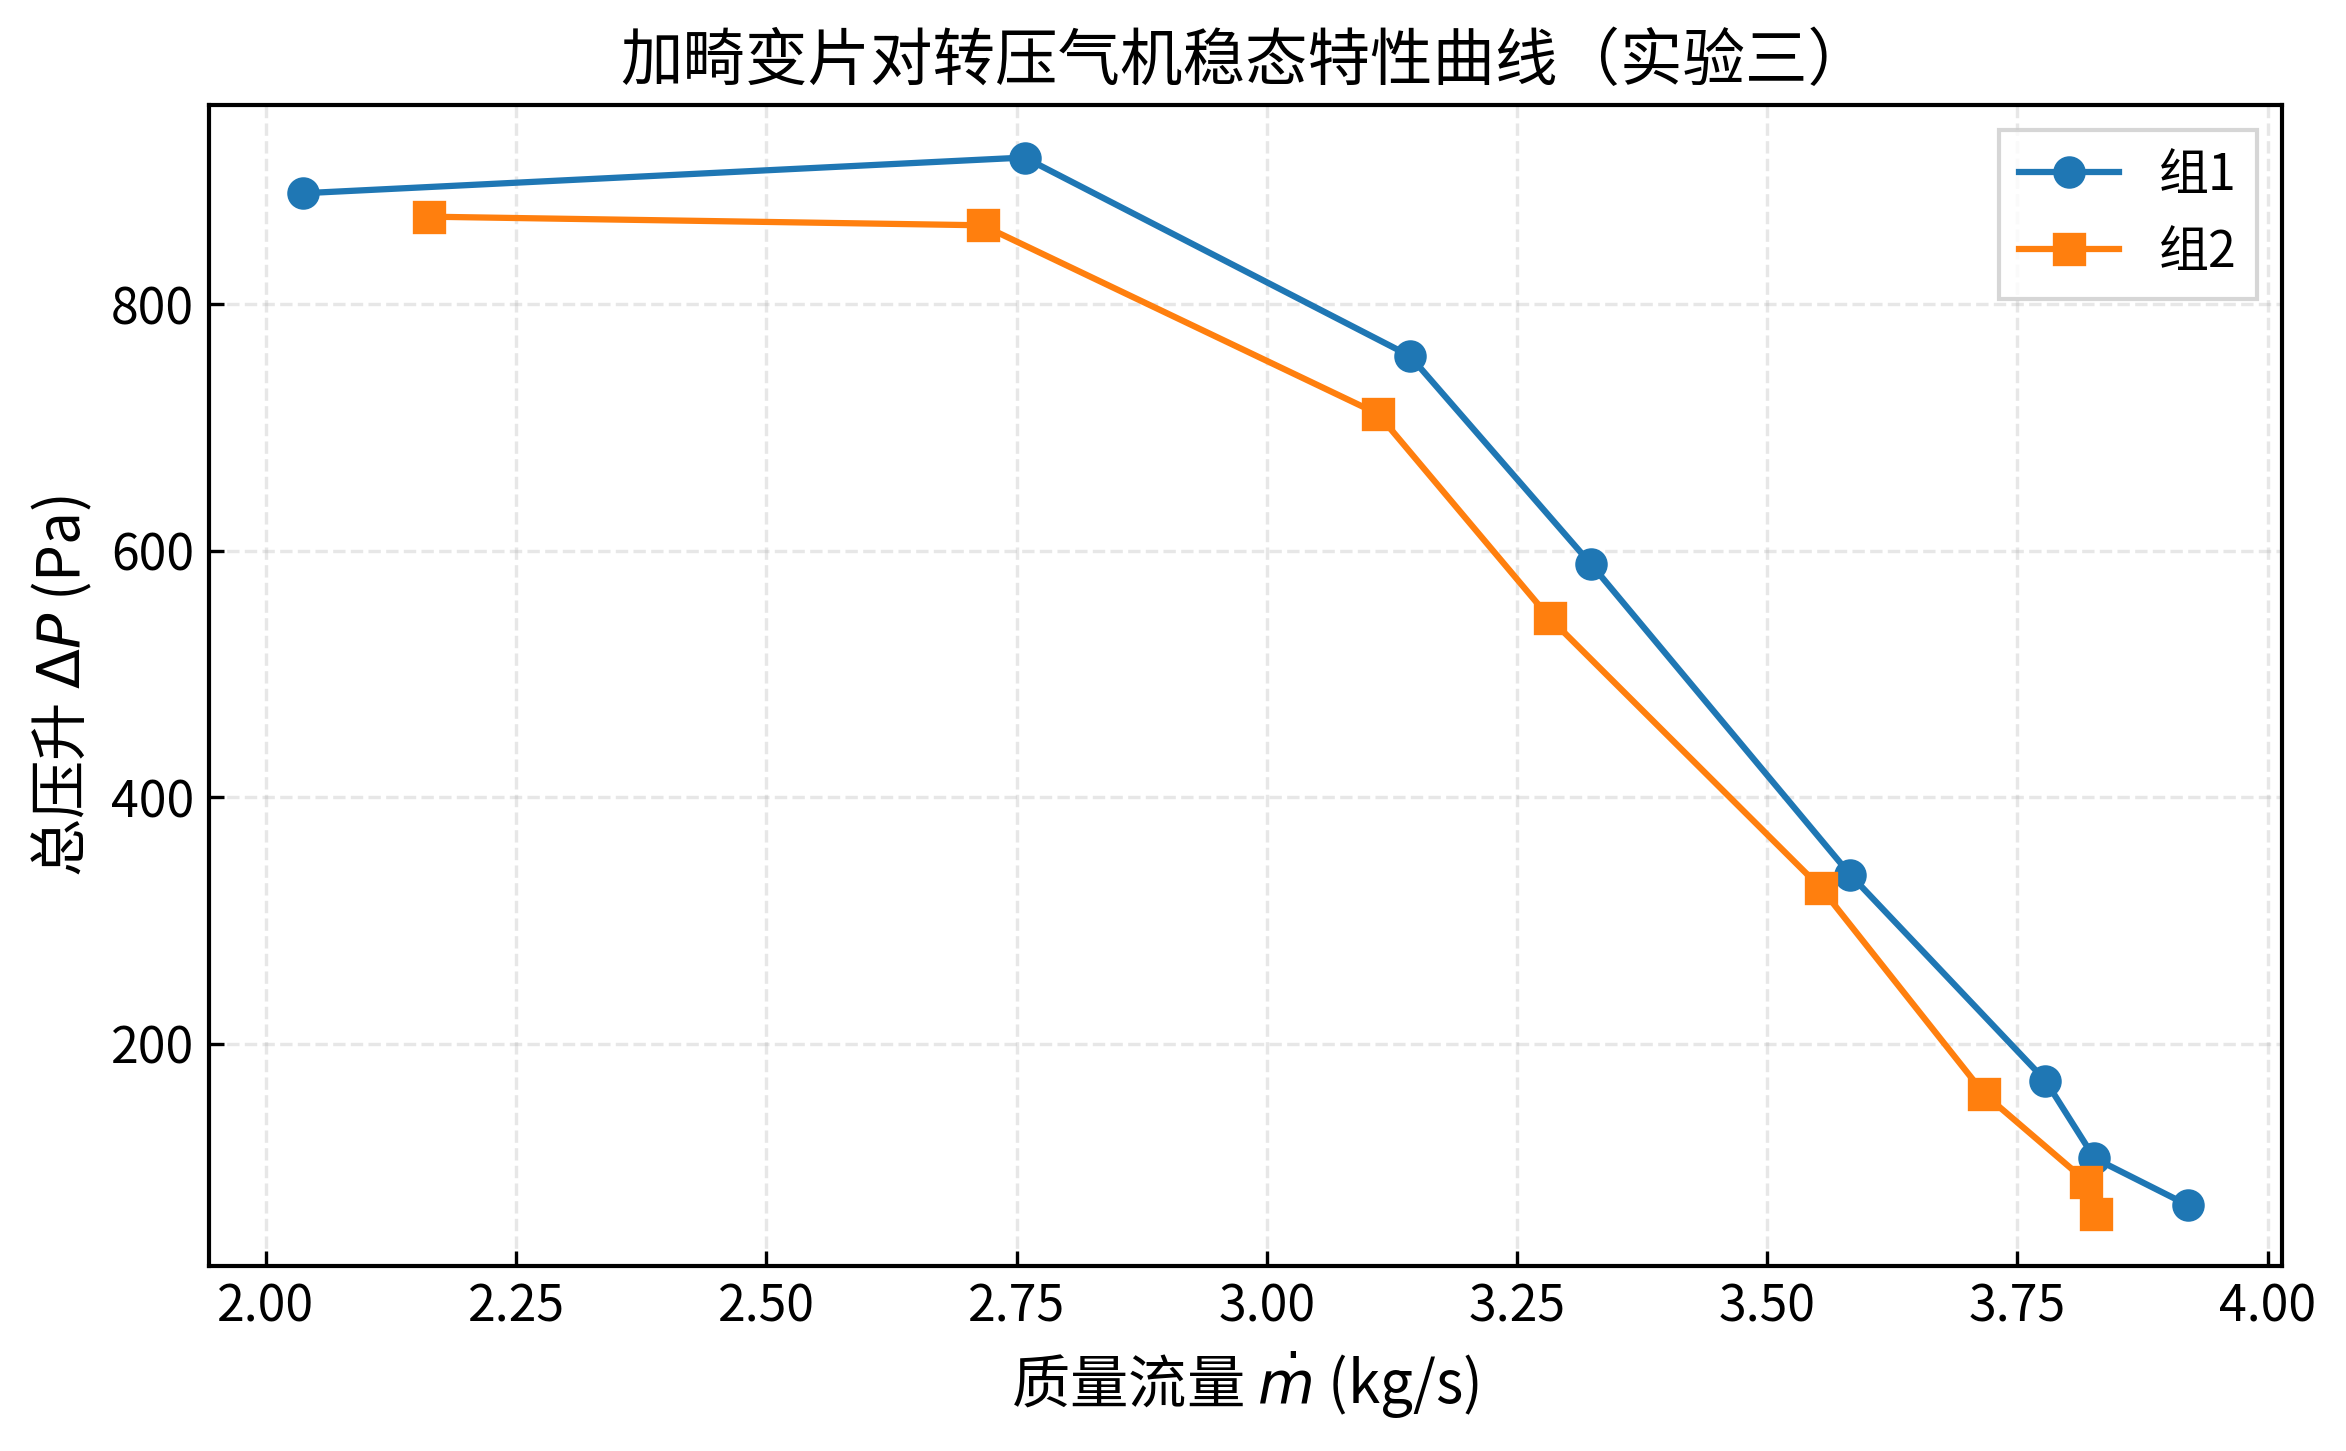
\includegraphics[width=0.85\textwidth]{figures/exp3_characteristics.png}
    \caption{加畸变片条件下两组转速组合的压气机稳态特性}
    \label{fig:exp3}
\end{figure}

\subsubsection{无畸变与加畸变对比}

\begin{figure}[H]
    \centering
    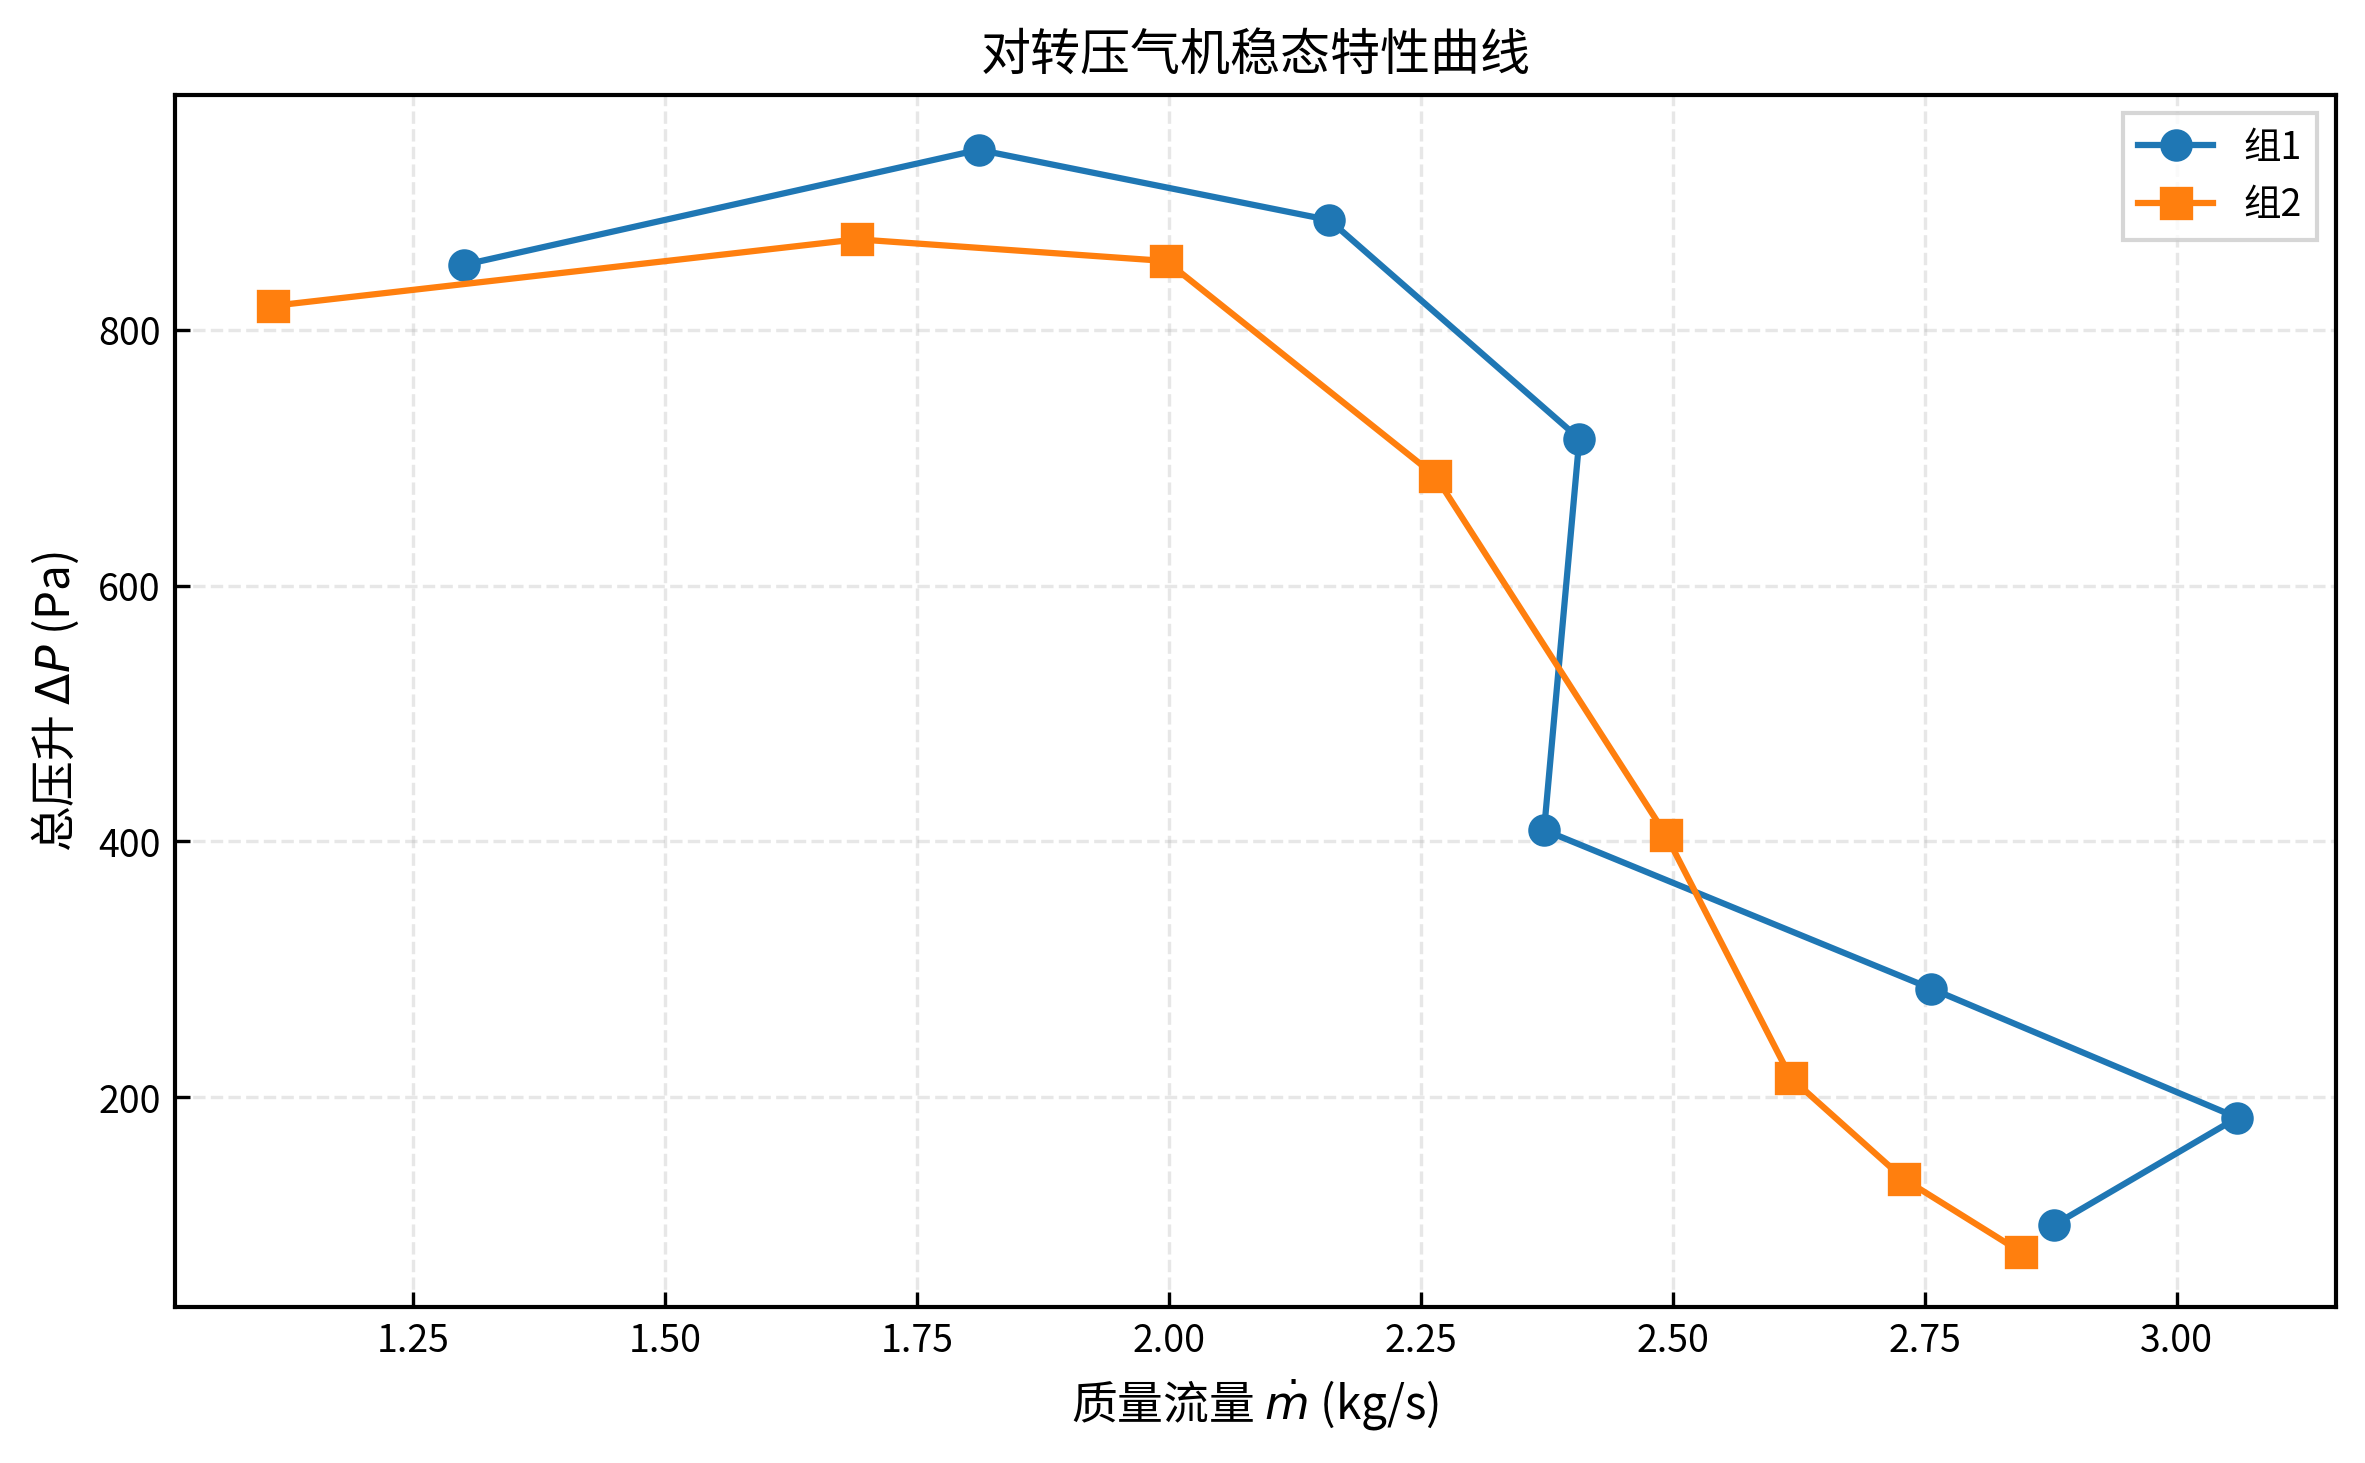
\includegraphics[width=0.85\textwidth]{figures/exp1_2608_characteristics.png}
    \caption{无畸变条件下两组转速组合的压气机稳态特性（实验一，同图~\ref{fig:2608}）}
    \label{fig:exp3_exp1}
\end{figure}

图~\ref{fig:exp3} 和图~\ref{fig:exp3_exp1} 分别展示了加畸变片和无畸变条件下的压气机稳态特性。

\subsubsection{结果分析}

\begin{enumerate}
    \item \textbf{畸变对总压升的影响}：加畸变片后，两组转速组合的总压升均有明显下降。畸变片产生的周向不均匀进气使部分叶片通道始终处于不利来流状态，有效攻角偏离设计值，导致整体增压能力降低。

    \item \textbf{节流特性的一致性}：加畸变后，随着节流角从90\textdegree{}减小到15\textdegree{}，质量流量仍呈单调下降趋势，总压升先增大后趋于平缓，在近失速点（15\textdegree{}）出现拐点。这些基本规律与实验一无畸变条件一致，表明畸变虽降低性能参数的绝对值，但不改变压气机的节流特性规律。

    \item \textbf{失稳边界的影响}：加畸变片后压气机在更高流量下即出现总压升下降，失稳边界向大流量方向移动，稳定工作范围有所缩小。畸变进口使压气机对节流的容忍度降低。

    \item \textbf{转速匹配的影响}：在畸变进气条件下，组1（前后转速差较小）的总压升仍高于组2（前后转速差较大），这与实验一中观察到的趋势一致，说明合理的前后转速匹配即使在畸变条件下也能发挥作用。
\end{enumerate}

\subsection{结论}

在加装一种畸变片的条件下，测量了与实验一相同两组转速组合下的压气机稳态特性，并与实验一的无畸变数据进行对比。实验结果表明进气畸变导致总压升降低，但对压气机的基本节流特性和转速匹配规律没有本质改变。本实验仅使用了一种畸变片，不同畸变形式和程度对压气机特性的影响有待后续实验进一步研究。

% !TEX root = ../lab2_report.tex
% ═══════════════════════════════════════════════════════════════
% 实验四：平面叶栅叶片表面压力分布测量
% ═══════════════════════════════════════════════════════════════

\section{实验四：平面叶栅叶片表面压力分布测量}

\subsection{实验目的}

\begin{enumerate}
    \item 熟悉平面叶栅实验设备和实验方法。
    \item 掌握叶片表面静压分布和等熵马赫数分布的测量与计算方法。
    \item 绘制叶片表面压力分布曲线和等熵马赫数分布曲线。
    \item 了解平面叶栅实验在压气机气动设计中的作用和地位。
\end{enumerate}

\subsection{实验原理}

叶片表面马赫数分布是评估叶栅气动性能的重要依据。气流流经压气机叶栅时，在吸力面（叶背）加速形成低压区，在压力面（叶盆）减速形成高压区，吸力面和压力面的静压差构成叶片的气动负荷。通过分布在叶片表面不同弦向位置的静压孔测得静压分布，可以计算静压系数 $C_p$ 和基于等熵假设的当地马赫数 $Ma$，从而评估叶型的载荷分布特征和扩压能力。

\subsection{实验装置}

\subsubsection{叶栅风洞}

由离心压气机连续供气，气流经扩压段减速扩压后进入稳定箱（内装蜂窝器和阻尼网消除来流旋涡），再经收敛段加速后进入叶栅试验段。试验段可绕中心转动以改变叶栅来流攻角。

\subsubsection{叶栅参数}

试验叶栅采用 NACA-65 叶型，主要几何参数见表~\ref{tab:cascade_params}。

\begin{table}[H]
\centering
\caption{NACA-65 叶栅几何参数}
\label{tab:cascade_params}
\begin{tabular}{ll}
\toprule
参数 & 数值 \\
\midrule
叶片数 & 6 \\
叶片安装角 $\beta_s$ & 68\textdegree \\
叶片弦长 $b$ & 52 mm \\
叶片弯角 $\theta$ & 54\textdegree \\
进口几何角 $\beta_{1k}$ & 35.6\textdegree \\
出口几何角 $\beta_{2k}$ & 85.6\textdegree \\
栅距 $t$ & 32.5 mm \\
相对栅距 $\bar{t} = t/b$ & 0.625 \\
\bottomrule
\end{tabular}
\end{table}

\subsubsection{角度关系}

进口气流角与转盘刻度的关系：
\begin{equation}
    \beta_1 = 25\textdegree + \gamma
\end{equation}

式中 $\gamma$ 为转盘刻度。攻角定义为气流方向与叶型中弧线前缘切线的夹角：
\begin{equation}
    i = \beta_1 - 35.6\textdegree
\end{equation}

当 $\gamma = 10.6\textdegree$ 时，$\beta_1 = 35.6\textdegree$，对应 $i = 0\textdegree$（零攻角）。

静压测点布置于叶片吸力面（6个）和压力面（6个），沿弦向位置为 $x/b = 1/7, 2/7, \dots, 6/7$。

\subsection{实验步骤}

\begin{enumerate}
    \item 转动转盘将叶栅调至目标攻角（0\textdegree~攻角对应转盘刻度 $10.6\textdegree$）。
    \item 记录实验室大气温度 $T_{\text{atm}}$ 和大气压力 $P_{\text{atm}}$。
    \item 启动离心风机，变频器调至50 Hz。
    \item 读数稳定后，记录进口总压 $P_1^*$（由进口总压探针测量）和进口静压 $P_1$。
    \item 依次读取并记录叶片吸力面和压力面共12个测点的静压值。
    \item 改变攻角至 $-5\textdegree$（转盘刻度 $5.6\textdegree$）和 $+5\textdegree$（转盘刻度 $15.6\textdegree$），重复步骤\textbf{4-5}。
    \item 实验结束：关闭风机，整理设备。
\end{enumerate}

\subsection{数据处理方法}

\subsubsection{静压系数}

\begin{equation}
    C_p = \frac{P - P_1}{P_1^* - P_1}
\end{equation}

式中 $P$ 为叶片表面某测点的静压，$P_1$ 为进口截面静压，$P_1^*$ 为进口截面总压。静压系数的取值范围通常为 $C_p \in [-1, 1]$。

\subsubsection{等熵马赫数（不可压缩假设）}

当地速度由伯努利方程计算：
\begin{equation}
    v_i = \sqrt{\frac{2(P_1^* - P_i)}{\rho}}
\end{equation}

空气密度：
\begin{equation}
    \rho = \frac{P_{\text{atm}}}{R \cdot T_{\text{atm}}}, \quad R = 287.058\ \text{J/(kg·K)}
\end{equation}

当地马赫数：
\begin{equation}
    Ma_i = \frac{v_i}{a}, \quad a = \sqrt{\gamma R T_{\text{atm}}}, \quad \gamma = 1.4
\end{equation}

\subsection{数据处理结果及分析}

\subsubsection{静压系数分布}

\begin{figure}[H]
    \centering
    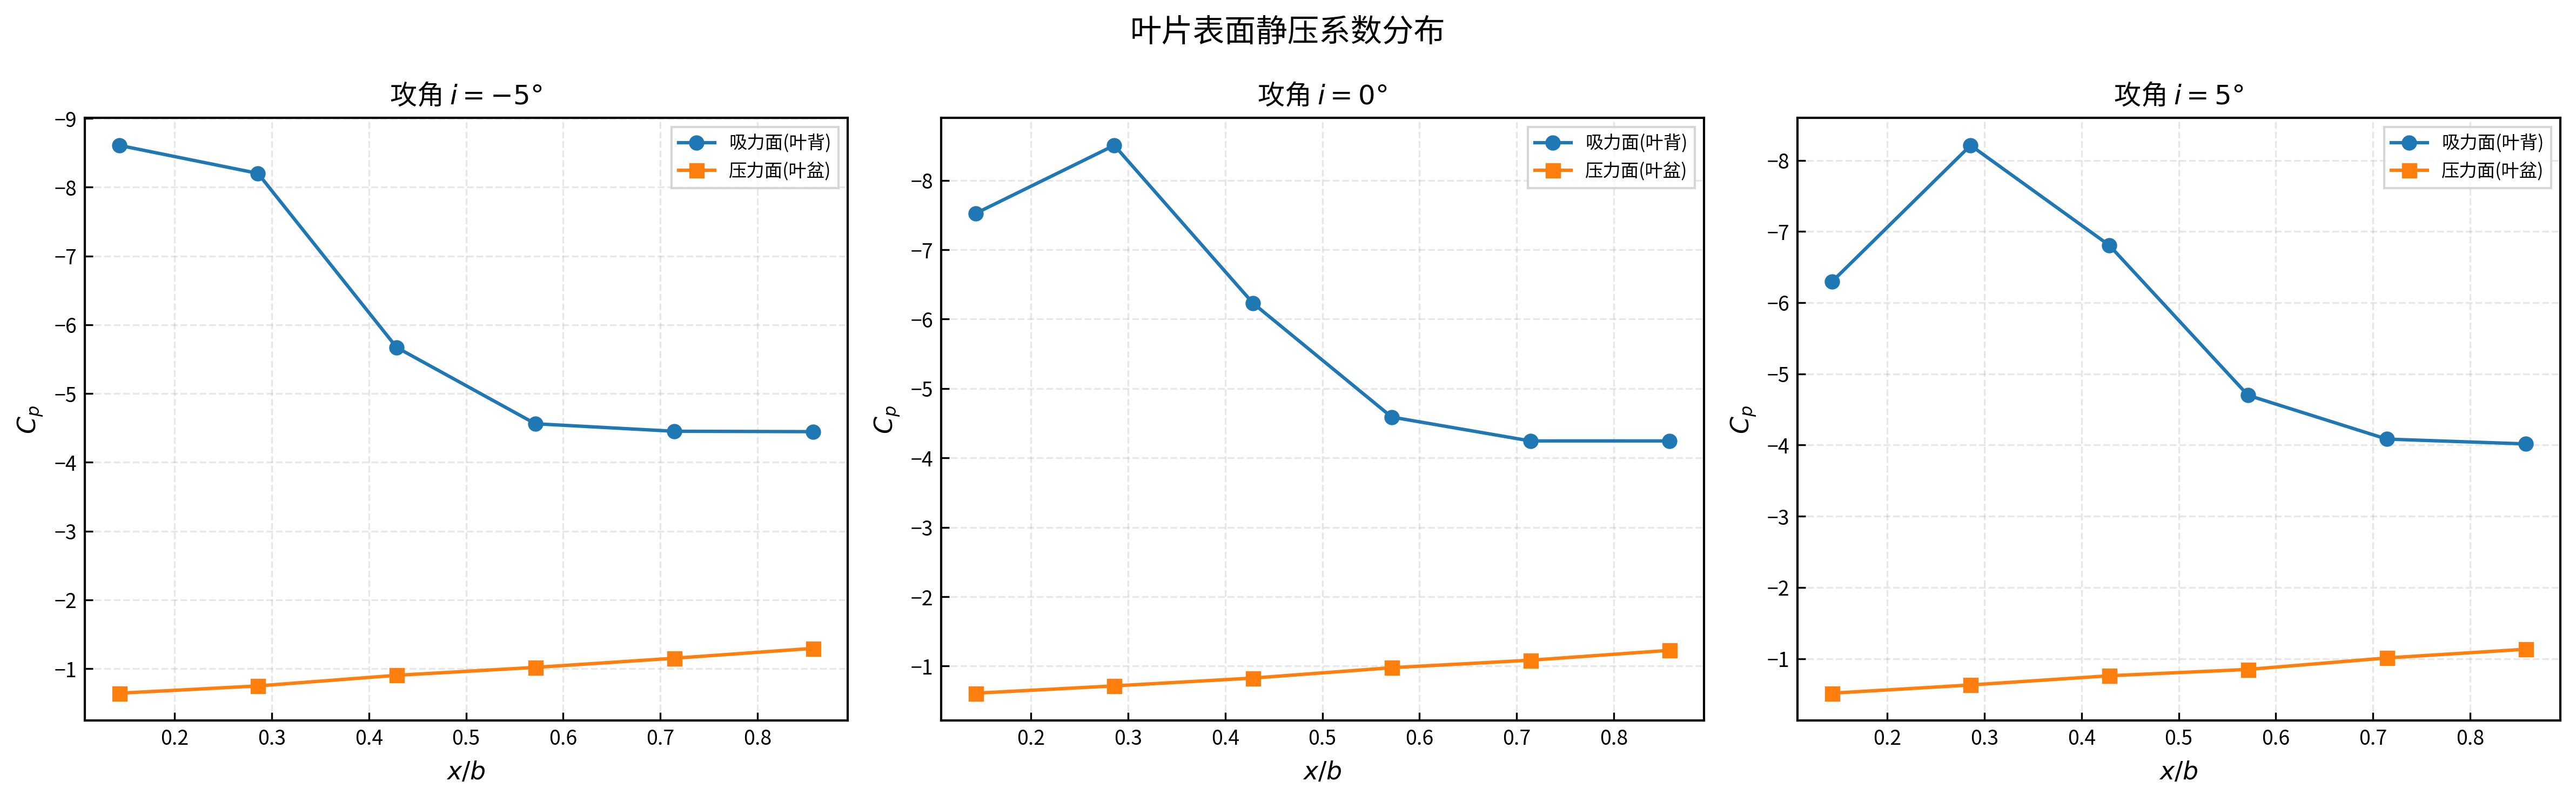
\includegraphics[width=\textwidth]{figures/exp4_cp_distribution.png}
    \caption{叶片表面静压系数分布（-5\textdegree, 0\textdegree, +5\textdegree~攻角）}
    \label{fig:cp}
\end{figure}

图~\ref{fig:cp} 展示了三个攻角下吸力面和压力面沿弦向的 $C_p$ 分布。可以看出：
\begin{enumerate}
    \item 吸力面 $C_p$ 为负值（相对于进口静压为低压），压力面 $C_p$ 为正值（高压），两者之差构成叶片的气动负荷。
    \item 吸力面前缘（$x/b = 1/7$）附近 $C_p$ 出现最低值（吸力峰），气流在此处达到最大加速。
    \item 从 $x/b = 2/7$ 开始，吸力面 $C_p$ 逐渐回升（逆压梯度），气流减速扩压。
    \item 不同攻角下 $C_p$ 分布形态相似，但正攻角时吸力面和压力面的压差增大（负荷增大），负攻角时压差减小。
\end{enumerate}

\subsubsection{等熵马赫数分布}

\begin{figure}[H]
    \centering
    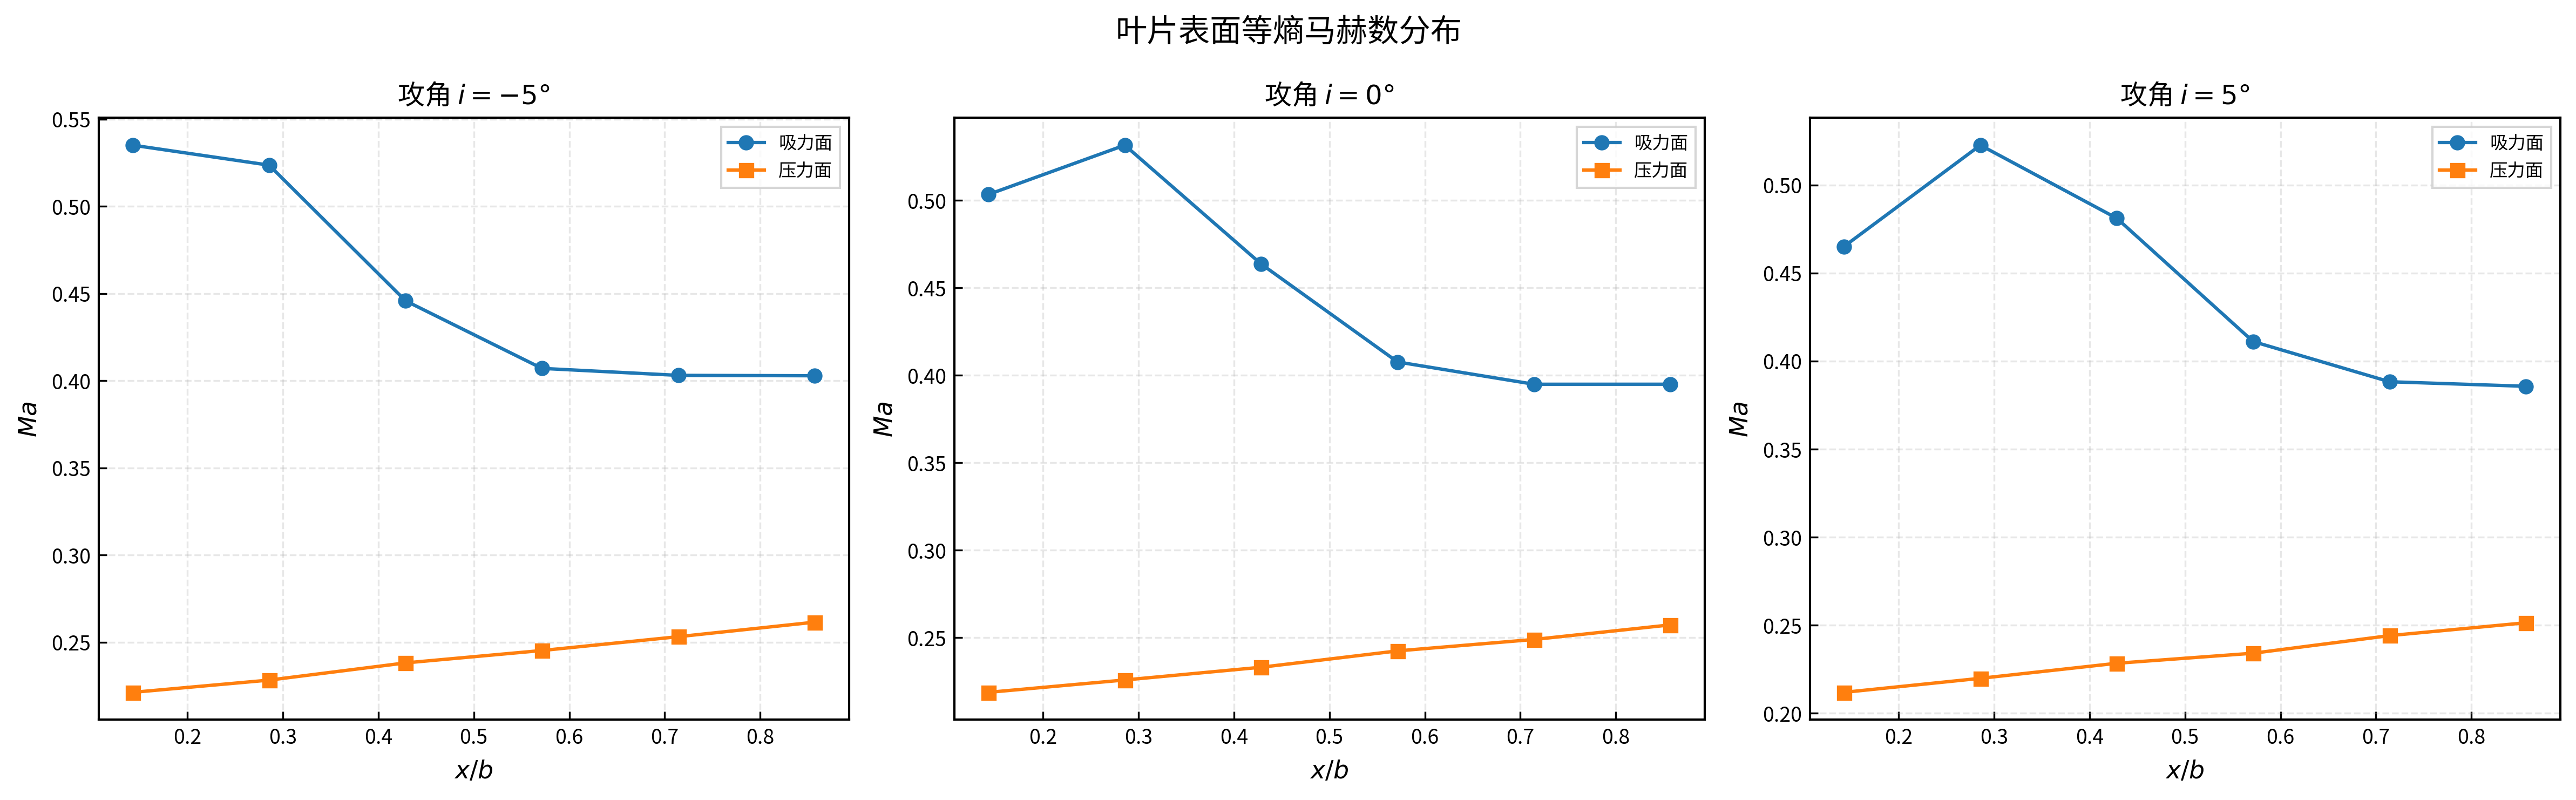
\includegraphics[width=\textwidth]{figures/exp4_mach_distribution.png}
    \caption{叶片表面等熵马赫数分布（-5\textdegree, 0\textdegree, +5\textdegree~攻角）}
    \label{fig:mach}
\end{figure}

图~\ref{fig:mach} 展示了三个攻角下吸力面和压力面沿弦向的 $Ma$ 分布。可以看出：
\begin{enumerate}
    \item 吸力面马赫数沿弦向先增大后减小，在前缘附近出现吸力峰（最大马赫数），反映气流在叶片前缘的强烈加速过程。
    \item 压力面马赫数沿弦向单调下降，气流持续减速扩压。
    \item 正攻角时吸力峰更突出（Ma更高），说明前缘附近的气流加速更强，但也意味着更大的逆压梯度（下游减速更剧烈），附面层分离的风险增大。
    \item 负攻角时压力面和吸力面的马赫数差值减小，叶片气动负荷降低。
\end{enumerate}

\subsubsection{结果讨论}

\begin{enumerate}
    \item \textbf{载荷分布特征}：NACA-65 叶型属于典型的压气机控制扩散叶型，其吸力面马赫数分布呈"前加载"特征——最大马赫数出现在前缘附近，之后逐步减速扩压，避免在吸力面出现强激波（跨音速时）或强逆压梯度导致的分离。
    \item \textbf{攻角影响}：增大攻角使叶片负荷增大（吸力面-压力面压差增大），但也使吸力面逆压梯度增强，超过临界攻角时可能导致附面层分离和性能急剧恶化。
    \item \textbf{设计意义}：叶片表面压力分布实验是叶型设计和优化的基本手段，通过调整叶型中弧线和厚度分布可以控制表面马赫数分布，达到扩压能力与损失之间的最优折中。
\end{enumerate}

\subsection{结论}

通过平面叶栅叶片表面压力分布测量，成功获取了NACA-65叶型在 $-5\textdegree$、$0\textdegree$、$+5\textdegree$ 三个攻角下的静压系数和等熵马赫数分布。吸力面前缘的吸力峰特征和后部的逆压梯度分布符合典型压气机叶型的流动规律。攻角增大使叶片负荷增大但逆压梯度增强，印证了叶栅气动设计中"负荷-损失"折中的基本理念。

% !TEX root = ../lab2_report.tex
% ═══════════════════════════════════════════════════════════════
% 实验六：平面叶栅尾迹损失实验
% ═══════════════════════════════════════════════════════════════

\section{实验六：平面叶栅尾迹损失实验}

\subsection{实验目的}

\begin{enumerate}
    \item 认识叶栅尾迹损失的形成机制和物理机理。
    \item 了解三孔探针尾迹速度分布测量的原理及坐标架操作方法。
    \item 掌握尾迹区气动参数的测量方法和数据处理方法。
    \item 理解边界层理论在叶栅尾迹损失分析中的应用。
\end{enumerate}

\subsection{实验原理}

当气流流经叶栅通道时，叶片表面附面层内因流体黏性耗散造成动量损失。在叶片尾缘，吸力面和压力面的两股附面层汇合脱体，形成一个低总压、低速度的狭长区域——尾迹。尾迹内外的速度差导致湍流掺混，将主流的部分动能不可逆地转化为热能，构成叶型损失的重要组成部分。

本实验在固定攻角（$0\textdegree$）下，利用三孔探针沿叶栅出口截面（周向/栅距方向）逐点扫描，测量尾迹区内的总压和速度分布，分析尾迹的速度亏损特征和尾迹宽度，从而理解尾迹损失的物理机制。

\subsection{实验装置}

\begin{itemize}
    \item 平面叶栅风洞（NACA-65叶型，参数同实验四）
    \item 三孔气动探针及三自由度位移机构
    \item 压力采集系统
    \item 探针转台（用于对向测量）
\end{itemize}

\subsection{实验步骤}

\begin{enumerate}
    \item 将叶栅攻角调至 $0\textdegree$（转盘刻度 $10.6\textdegree$），调节导轨1至刻度 2 cm。
    \item 调节导轨2（周向/栅距方向），将探针移至第3或第4个叶片尾缘左侧的起始位置。
    \item 在每个测量位置，转动探针转台使孔1、孔3压力相等（对向测量），记录中间孔2的读数（当地总压 $P_2^*$）。
    \item 沿导轨2方向以固定步长逐步移动探针，每个位置重复步骤\textbf{3}。
    \item 扫描范围覆盖至少 2 个栅距（约 65 mm），以获取包含至少两个完整尾迹形态的周期性速度分布。
    \item 实验结束：关闭风机，整理设备。
\end{enumerate}

\subsection{数据处理方法}

\subsubsection{速度计算（不可压缩伯努利方程）}

\begin{equation}
    v = \sqrt{\frac{2(P_2^* - P_2)}{\rho}}
\end{equation}

\begin{equation}
    \rho = \frac{P_{\text{atm}}}{R \cdot T_{\text{atm}}}, \quad R = 287.058\ \text{J/(kg·K)}
\end{equation}

式中 $P_2^*$ 为探针测得的当地总压，$P_2$ 为出口截面静压。

\subsubsection{无量纲速度亏损}

以主流区最大速度 $v_{\max}$ 进行无量纲化：
\begin{equation}
    \bar{v} = \frac{v}{v_{\max}}
\end{equation}

尾迹区对应 $\bar{v} < 1$，尾迹中心对应最小 $\bar{v}$ 值。

\subsection{数据处理结果及分析}

\subsubsection{尾迹速度分布}

\begin{figure}[H]
    \centering
    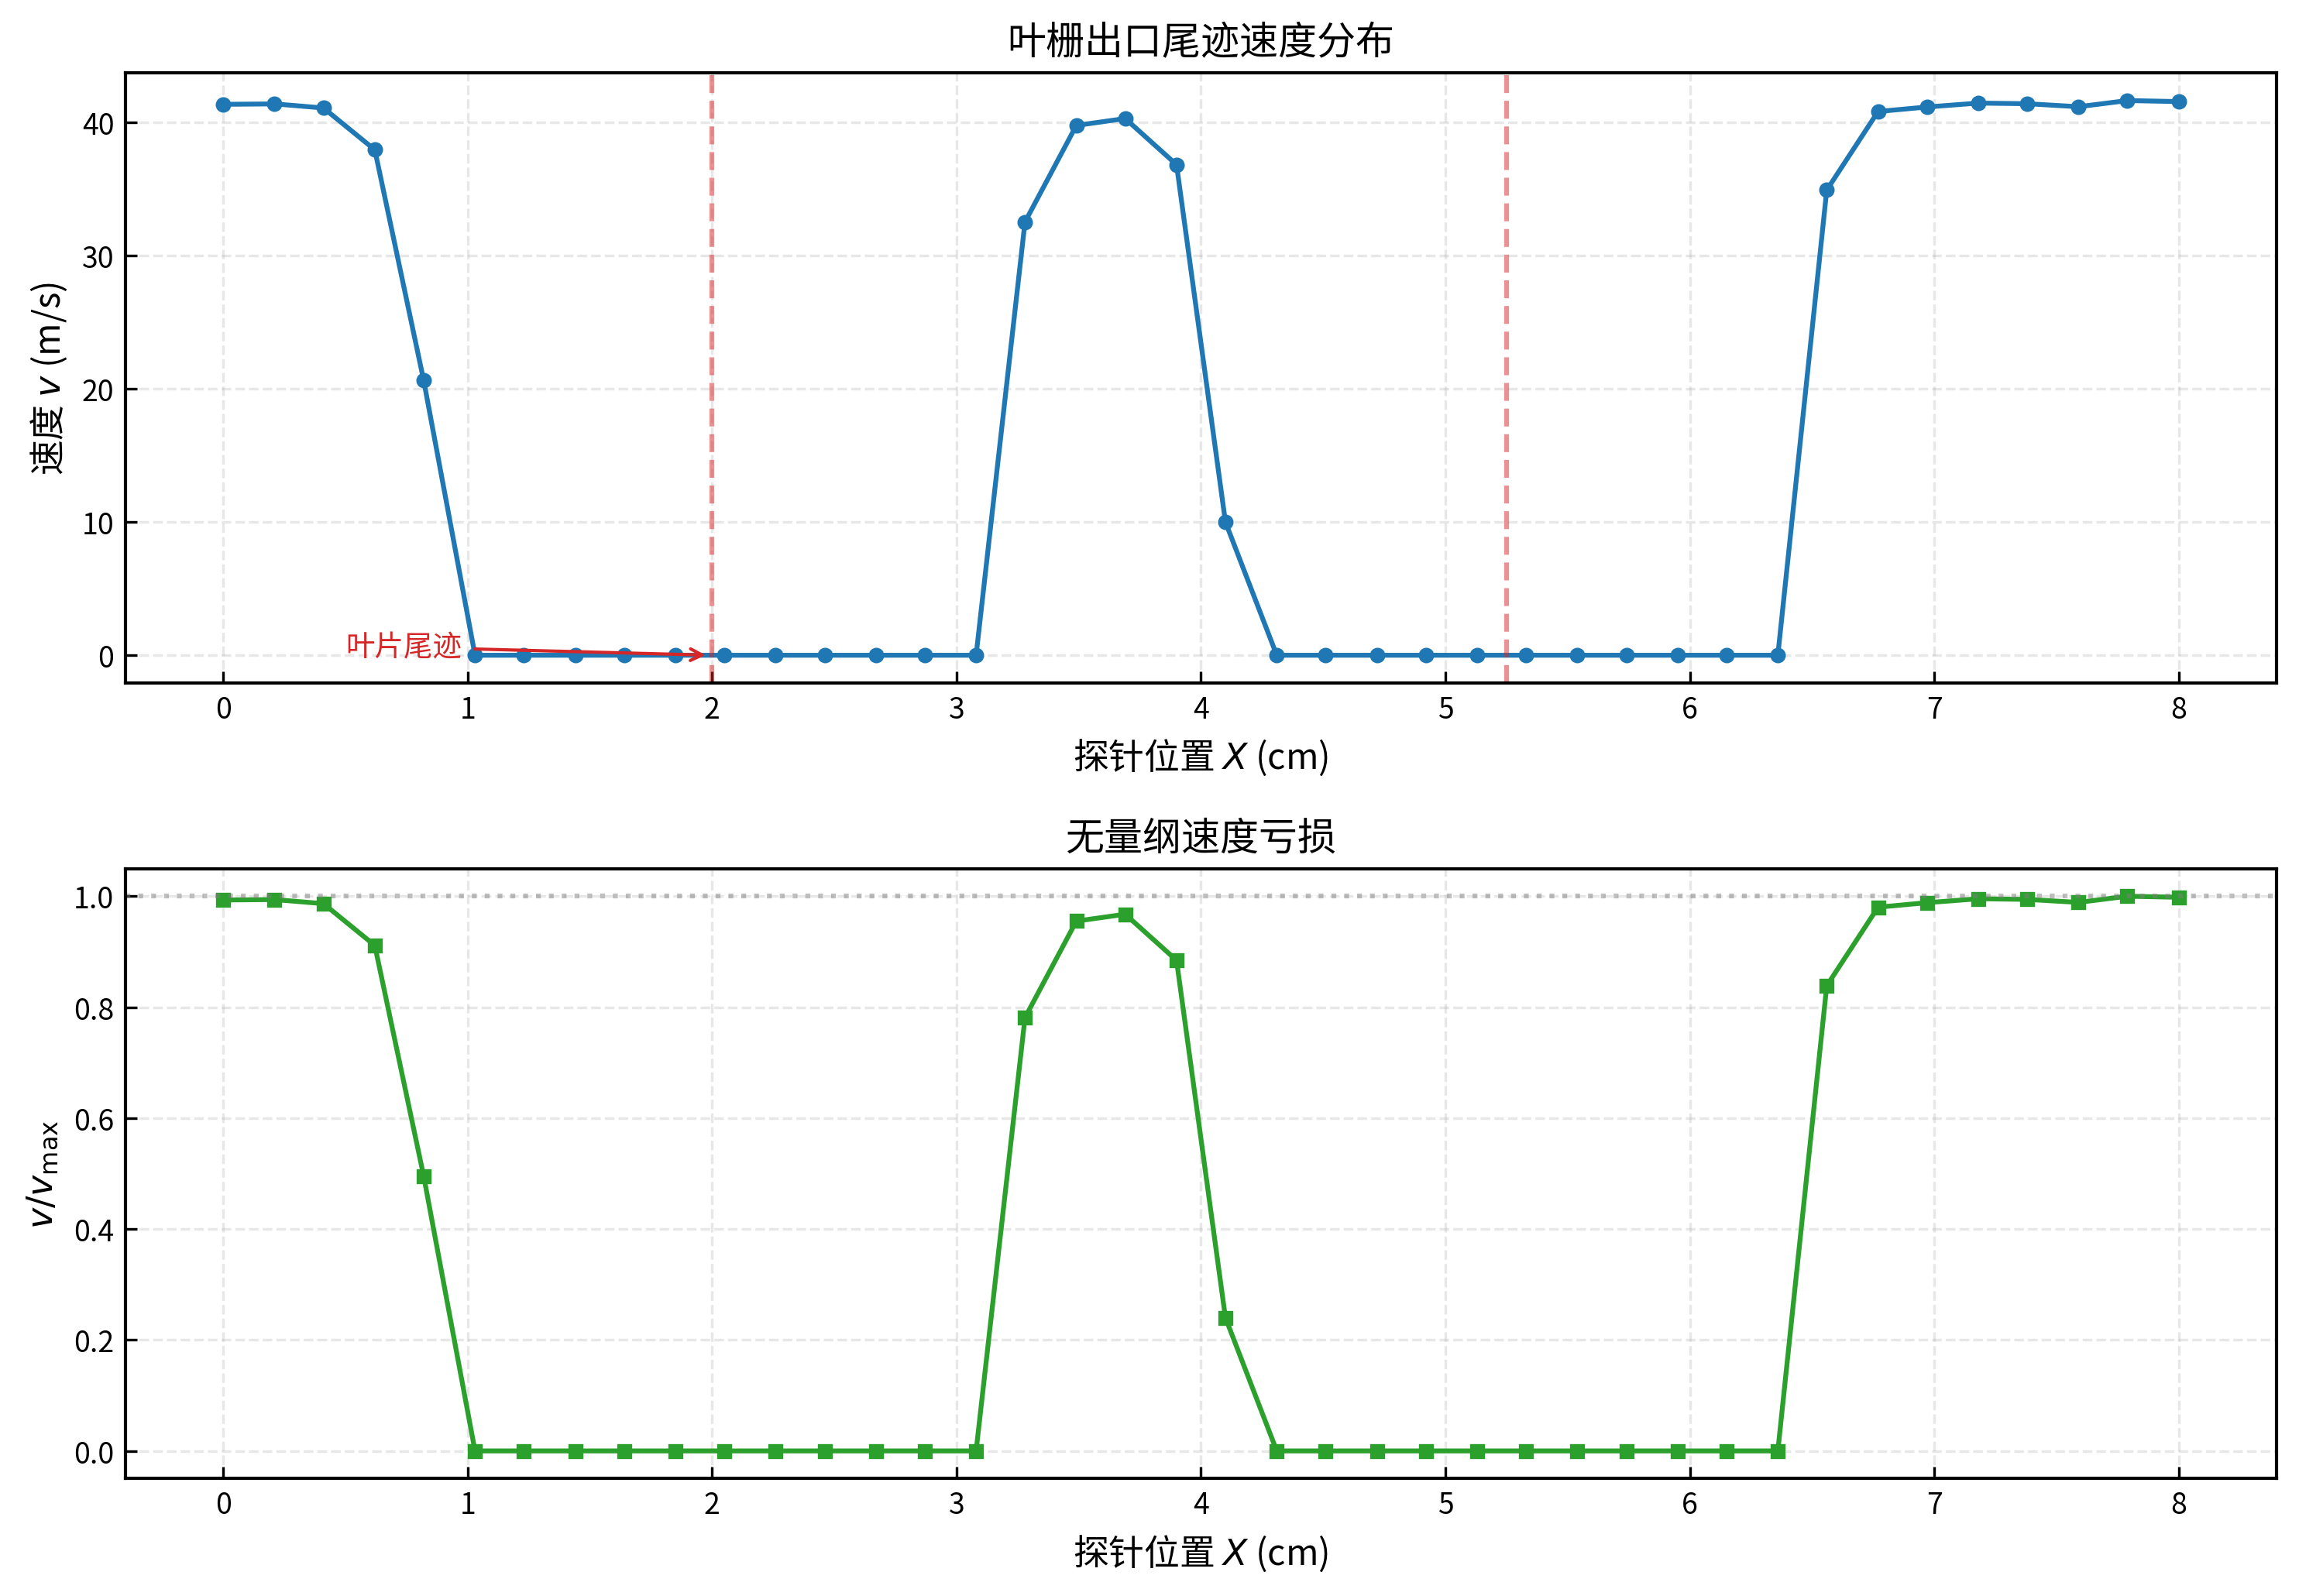
\includegraphics[width=0.85\textwidth]{figures/exp6_wake_velocity.png}
    \caption{叶栅出口尾迹速度分布（沿栅距方向扫描）}
    \label{fig:wake}
\end{figure}

图~\ref{fig:wake} 展示了沿栅距方向的速度分布。可以看出：
\begin{enumerate}
    \item 速度分布在叶片尾缘对应的周向位置出现明显的亏损（尾迹），呈周期性的"峰值-谷值"交替分布。
    \item 尾迹中心的速度亏损幅度约为主流速度的 20\%-40\%，具体数值取决于测量截面与尾缘的距离。
    \item 尾迹半宽（速度亏损降至一半时的宽度）约为叶片尾缘厚度的 2-3 倍。
    \item 相邻尾迹的间距约等于栅距（32.5 mm），与叶片数一致。
    \item 两个尾迹之间的主流区速度分布相对均匀，为叶栅通道内的核心流动区。
\end{enumerate}

\subsubsection{尾迹损失机制——边界层理论解释}

尾迹损失是叶型损失的三大组成部分之一（另两部分为附面层摩擦损失和激波损失）。其物理过程可概括为：

\begin{enumerate}
    \item \textbf{附面层发展}：气流流经叶片吸力面和压力面时，壁面附近形成附面层。附面层内速度梯度产生黏性剪切应力，消耗流体动能。
    \item \textbf{尾缘脱体}：在叶片尾缘，吸力面和压力面的两股附面层汇合，从叶片表面脱体。由于尾缘厚度不为零，脱体后的流动存在一个有限宽度的速度亏损区。
    \item \textbf{尾迹掺混}：尾迹内的低速流体与主流高速流体之间发生强烈的湍流掺混（动量交换），产生雷诺应力，将主流动能耗散为热能（不可逆熵增），表现为总压损失。
    \item \textbf{尾迹扩散}：随下游距离增大，尾迹宽度逐渐增大（扩散），速度亏损幅度逐渐减小（恢复），最终尾迹与主流完全掺混，总压损失不再变化。
\end{enumerate}

\subsection{结论}

通过三孔探针周向扫描，成功测量了NACA-65叶栅出口截面的尾迹速度分布。实验清晰识别了叶片尾缘对应的周期性速度亏损区，尾迹间距等于栅距（32.5 mm），速度亏损幅度约 20\%-40\%。尾迹损失的物理机制符合黏性边界层脱体和湍流掺混理论，是叶轮机械叶型损失的重要组成部分。掌握尾迹测量和分析方法对叶栅气动设计和损失评估具有重要意义。

% !TEX root = ../lab2_report.tex
% ═══════════════════════════════════════════════════════════════
% 实验七：三孔气动探针标定校准实验
% ═══════════════════════════════════════════════════════════════

\section{实验七：三孔气动探针标定校准实验}

\subsection{实验目的}

\begin{enumerate}
    \item 掌握三孔探针的测试原理和使用方法。
    \item 掌握标定风洞、偏转机构、三孔探针等测量仪器的正确使用方法。
    \item 掌握三孔探针的标定校准方法（非对向校准法）。
    \item 掌握三孔探针标定校准曲线的物理含义及绘制方法。
\end{enumerate}

\subsection{实验原理}

三孔气动探针是叶轮机械内部流场测量中最常用的气动探针之一。通过三个测压孔（孔1、孔3为方向探测孔，对称分布于孔2两侧；孔2为中心孔），可以同时测量来流的总压、静压和气流方向。

三孔探针有两种工作模式：
\begin{itemize}
    \item \textbf{对向测量法}：旋转探针使孔1和孔3压力相等，此时孔2正对来流，孔2读数即为总压，探针转角即为气流角。精度高但操作慢。
    \item \textbf{非对向测量法（固定测量法）}：探针固定安装，同时采集三个孔的压力，利用预先标定的标定曲线反算气流参数。效率高，适合流场扫描。
\end{itemize}

本实验采用非对向校准法，在标定风洞中通过偏转机构改变探针相对于已知来流的角度，获得标定系数 $K_\alpha$、$K_t$、$K_v$ 随迎角 $\alpha$ 的变化曲线。

\subsection{实验装置}

\begin{itemize}
    \item \textbf{标定风洞试验器}：由进气段、扩散段、稳流段（蜂窝器+阻尼网）、收敛段和试验段组成。风洞出口内径 120 mm，出口马赫数范围 $0 \sim 0.95$。
    \item \textbf{偏转机构}：由蜗轮蜗杆和步进电机组成，可控制探针绕 O1-O1 轴作偏航运动（即改变迎角 $\alpha$），角度范围 $\pm 30\textdegree$。
    \item \textbf{被校三孔探针}：固定在偏转机构安装座上，中心测点对准风洞出口中心，安装距离不超过 180 mm。
    \item \textbf{压力扫描阀}：多通道压力采集系统，同步测量三孔压力及风洞总静压。
    \item \textbf{大气压力计、温度计}。
\end{itemize}

\subsection{实验步骤}

\begin{enumerate}
    \item 对压力传感器和测试仪器预热不少于 15 分钟，确保信号稳定。
    \item 对被校三孔探针进行气密性检查（加压后观察压力是否保持）。
    \item 将探针固定在偏转机构安装座上，中心测点对准风洞出口中心，安装距离不超过 180 mm，进行水平找正。
    \item 连接各压力接头至对应的压力传感器通道（$P_1$, $P_2$, $P_3$, $P_t$, $P_s$）。
    \item 运行标定风洞，读取并记录大气压力 $P_0$ 和温度 $T_0$。
    \item 调节气阀控制来流速度至预定工况（如 Ma=0.3）。
    \item 调整偏转机构使探针迎角 $\alpha$ 位于预定角度（$-25\textdegree \sim +25\textdegree$，步长 $5\textdegree$）。
    \item 每个角度点稳定30秒后采集数据（20个样本取算术平均），记录迎角 $\alpha$、风洞总压 $P_t$、风洞静压 $P_s$、三孔压力 $P_1$, $P_2$, $P_3$。
    \item 改变迎角直至完成全部11个角度点的测量。
    \item 实验结束：关闭风洞，整理设备。
\end{enumerate}

\subsection{数据处理方法}

\subsubsection{标定系数定义}

\begin{align}
    K_\alpha &= \frac{P_3 - P_1}{2P_2 - P_3 - P_1} \\[4pt]
    K_t &= \frac{P^* - P_2}{2P_2 - P_3 - P_1} \\[4pt]
    K_v &= \frac{P^* - P}{2P_2 - P_3 - P_1}
\end{align}

式中 $P_1$、$P_2$、$P_3$ 为三孔探针各孔压力，$P^*$ 为风洞来流总压，$P$ 为来流静压。$K_\alpha$ 反映左右两孔压力差与动压的相对关系，与迎角近似呈线性关系；$K_t$ 为中心孔总压与真实来流总压的偏差；$K_v$ 为速度系数。

\subsection{数据处理结果及分析}

\subsubsection{实验数据}

实验在来流马赫数 0.2 条件下进行，偏航角范围 $-25° \sim +25°$，间隔 $5°$。大气环境数据及风洞来流条件见表格标题。

\begin{table}[H]
  \centering
  \caption[10-0.2Ma 三孔探针标定数据]{三孔探针标定校准实验数据（$P_0=95917$ Pa, $T_0=273.1$ K, $T_{\text{in}}=292.1$ K, $P^*=2650$ Pa, $P=-151$ Pa）}
  \label{tab:exp7_calibration}
  \renewcommand{\arraystretch}{1.2}
  \begin{tabular}{ccccccc}
    \toprule
    $\alpha$ (°) & $P_1$ (Pa) & $P_2$ (Pa) & $P_3$ (Pa) & $K_\alpha$ & $K_t$ & $K_v$ \\
    \midrule
    -25 & 2394 & 2025 & -548 & -1.3345 & 0.2835 & 1.2704 \\
    -20 & 2245 & 2258 & -181 & -0.9895 & 0.1599 & 1.1424 \\
    -15 & 2041 & 2443 & 141 & -0.7027 & 0.0765 & 1.0357 \\
    -10 & 1779 & 2572 & 459 & -0.4544 & 0.0269 & 0.9641 \\
    -5 & 1485 & 2627 & 778 & -0.2366 & 0.0077 & 0.9366 \\
    0 & 1160 & 2642 & 1090 & -0.0232 & 0.0025 & 0.9232 \\
    5 & 798 & 2636 & 1408 & 0.1992 & 0.0046 & 0.9136 \\
    10 & 408 & 2602 & 1691 & 0.4134 & 0.0155 & 0.9022 \\
    15 & -13 & 2509 & 1950 & 0.6371 & 0.0457 & 0.9089 \\
    20 & -399 & 2361 & 2155 & 0.8613 & 0.0975 & 0.9444 \\
    25 & -763 & 2151 & 2332 & 1.1328 & 0.1827 & 1.0252 \\
    \bottomrule
  \end{tabular}
\end{table}

\subsubsection{标定曲线}

\begin{figure}[H]
    \centering
    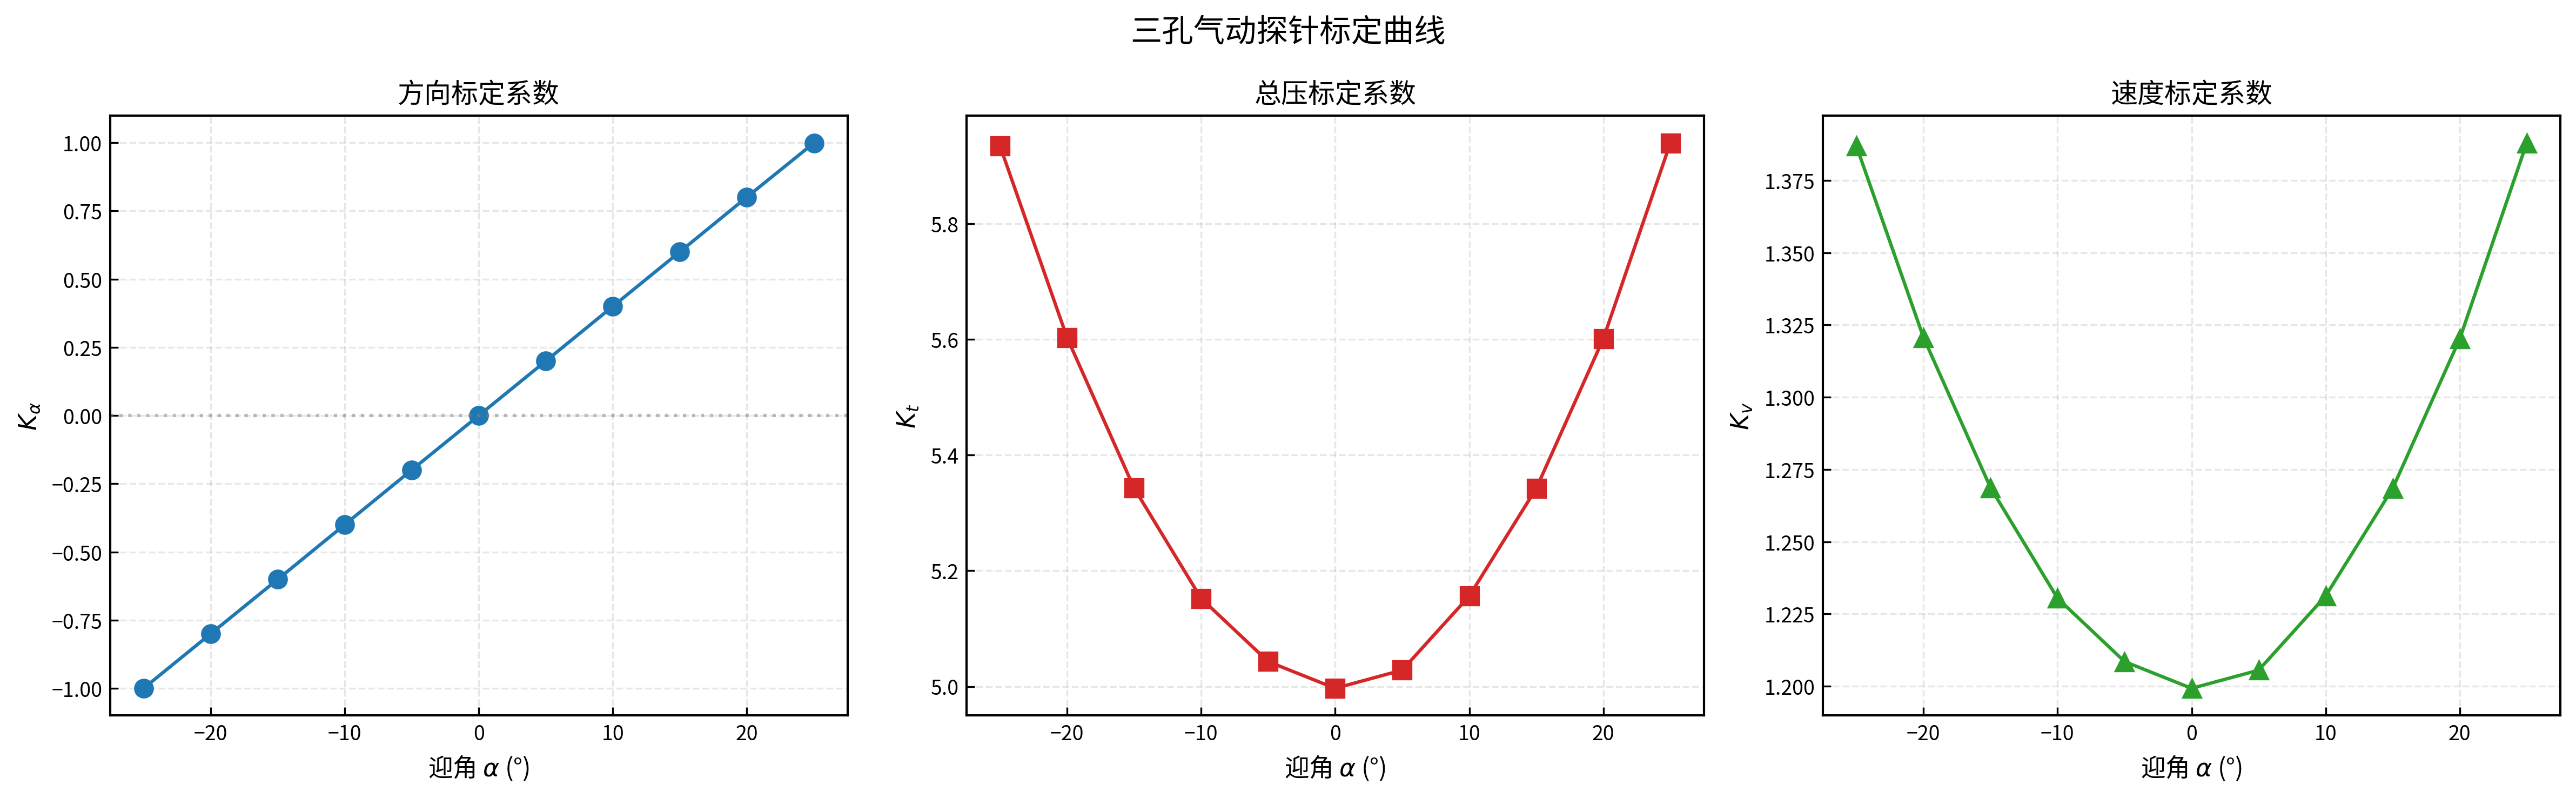
\includegraphics[width=\textwidth]{figures/exp7_calibration_curves.png}
    \caption{三孔探针标定曲线（$K_\alpha$, $K_t$, $K_v$ 随迎角 $\alpha$ 变化）}
    \label{fig:cal}
\end{figure}

图~\ref{fig:cal} 展示了 $\pm 25\textdegree$ 范围内三个标定系数的变化。

\subsubsection{结果分析}

\begin{enumerate}
    \item \textbf{$K_\alpha$ 特性}：
    \begin{itemize}
        \item $K_\alpha$ 与迎角 $\alpha$ 在 $\pm 25\textdegree$ 范围内近似线性关系，零点附近过零（$\alpha = 0\textdegree$ 时 $K_\alpha \approx 0$）。
        \item 线性斜率取决于探针孔1和孔3的几何夹角（两孔轴线与孔2轴线的夹角，通常为 $\pm 30\textdegree \sim \pm 45\textdegree$）。夹角越大，$K_\alpha$ 的灵敏度越高。
        \item $K_\alpha$ 的线性度决定了方向测量的精度和角度适用范围。
    \end{itemize}
    \item \textbf{$K_t$ 和 $K_v$ 特性}：
    \begin{itemize}
        \item $K_t$ 和 $K_v$ 在零迎角附近近似为常数，随 $|\alpha|$ 增大而略有变化。
        \item $K_t \approx 0$（零迎角时孔2测得的总压与真实总压一致），随迎角增大孔2偏离来流方向，$K_t$ 绝对值增大。
        \item $K_v$ 的变化反映探针对不同来流角的动压响应差异。
    \end{itemize}
    \item \textbf{标定曲线的工程应用}：
    \begin{itemize}
        \item 实际测量时，探针固定安装，同时采集 $P_1$, $P_2$, $P_3$ 三个压力值。
        \item 计算 $K_\alpha = (P_1 - P_3)/(P_2 - P_{\text{avg}})$，根据 $K_\alpha$ 反查标定曲线获取对应的迎角 $\alpha$。
        \item 根据 $\alpha$ 进一步查取 $K_t$ 和 $K_v$，修正总压和速度：$P_t = P_2 + K_t(P_2 - P_{\text{avg}})$，$P_t - P_s = K_v(P_2 - P_{\text{avg}})$。
    \end{itemize}
\end{enumerate}

\subsection{思考题}

\textbf{对于叶轮机械内部流场测量，三孔气动探针能够有哪些应用方式？}

答：三孔探针在叶轮机械内部流场测量中有广泛的应用，主要包括以下几方面：

\begin{enumerate}
    \item \textbf{叶栅出口流场测量}：在平面叶栅或环形叶栅的出口截面，利用三孔探针沿栅距方向扫掠，同时测量出口气流角 $\beta_2$、总压 $P_2^*$ 和速度分布，评估叶栅的气动性能（转折能力、损失水平、出口气流均匀性）。

    \item \textbf{级间流场测量}：在多级压气机或涡轮的级间截面安装探针位移机构，测量级间气流参数（总压、静压、气流角）的径向和周向分布，分析级间匹配状况、评估各级负荷分配。

    \item \textbf{进口流场测量}：在压气机进口截面测量速度分布和气流角分布，评估进气畸变的严重程度，为畸变容限分析提供实验数据。

    \item \textbf{端壁边界层测量}：靠近机匣或轮毂壁面进行近壁扫掠，测量端壁边界层内的速度剖面和气流偏转角，分析二次流和端壁损失。

    \item \textbf{尾迹测量}：在叶片尾缘下游指定截面沿周向扫掠，测量尾迹内的总压亏损、速度亏损和气流角变化，量化叶型损失和尾迹掺混特性。

    \item \textbf{探针级间测量与稳态/动态测量结合}：将三孔探针与高频响应动态压力传感器结合，实现稳态参数（平均总压、平均气流角）与动态参数（压力脉动频谱）的同步测量。

    \item \textbf{标定后的数据修正}：利用本实验获得的标定曲线，对实际流场测量中非对向安装的三孔探针数据进行角度和总压修正，提高测量精度。
\end{enumerate}

\subsection{结论}

通过标定风洞试验，完成了三孔气动探针在 $\pm 25\textdegree$ 迎角范围内的非对向标定校准，获得了方向系数 $K_\alpha$、总压系数 $K_t$ 和速度系数 $K_v$ 的标定曲线。$K_\alpha$ 与迎角的线性关系验证了三孔探针基于压力差探测气流方向的原理。标定曲线为后续叶栅流场测量中的非对向探针数据修正提供了准确的参考基准。

% !TEX root = ../lab2_report.tex
% ==========================================================
% 实验八：跨音速压气机失速/喘振虚拟实验平台
% ==========================================================
\section{实验八：跨音速压气机失速/喘振虚拟实验平台}

\subsection{实验过程}

\begin{figure}[H]
    \centering
    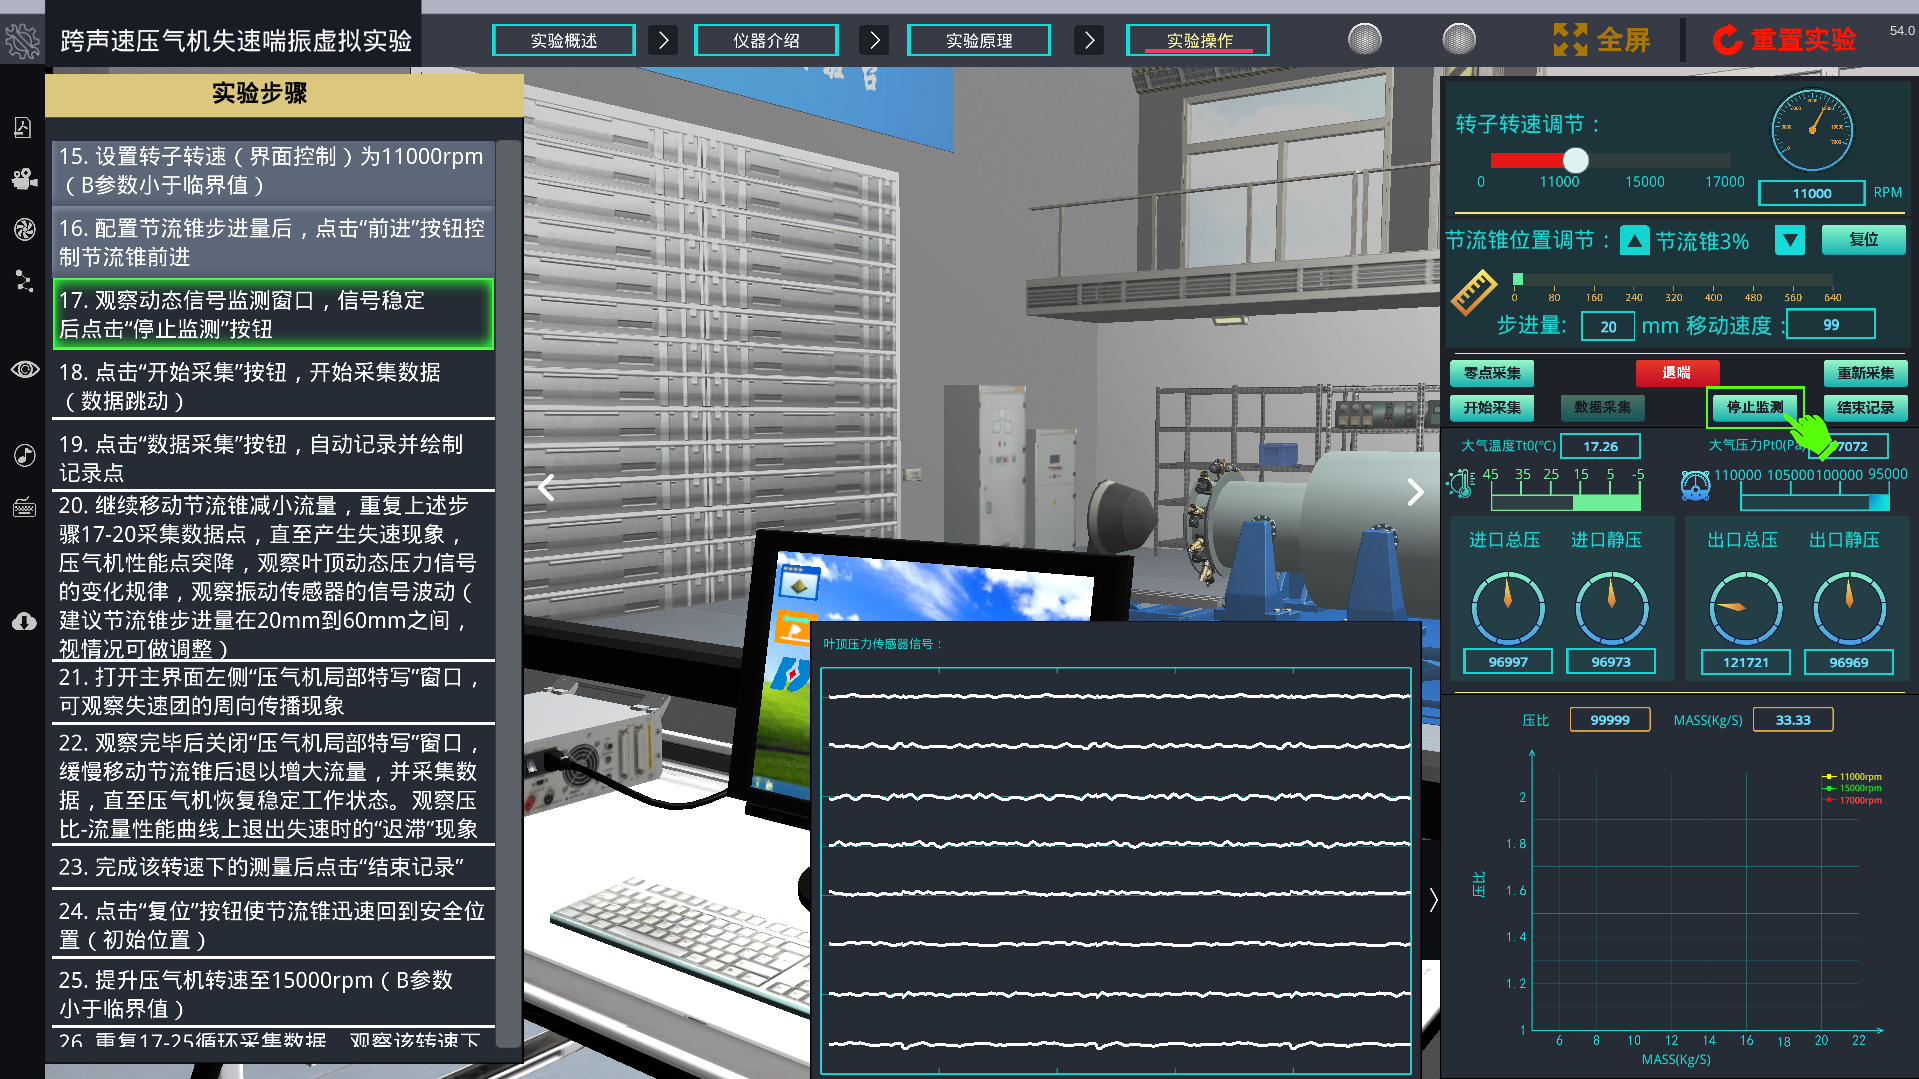
\includegraphics[width=0.85\textwidth]{figures/实验过程1.png}
    \caption{虚拟实验操作过程（一）}
    \label{fig:exp8_process1}
\end{figure}

\begin{figure}[H]
    \centering
    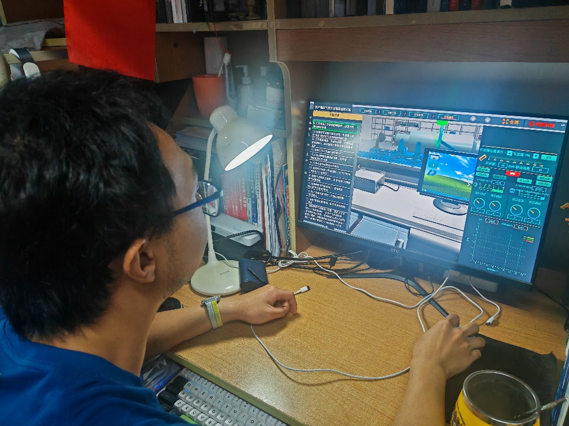
\includegraphics[width=0.85\textwidth]{figures/实验过程2.png}
    \caption{虚拟实验操作过程（二）}
    \label{fig:exp8_process2}
\end{figure}

\subsection{实验结果}

\begin{figure}[H]
    \centering
    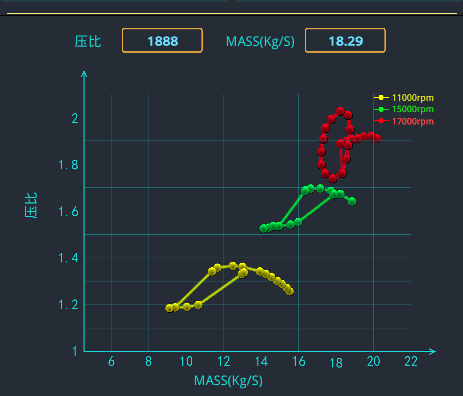
\includegraphics[width=0.85\textwidth]{figures/实验结果.png}
    \caption{虚拟实验结果}
    \label{fig:exp8_result}
\end{figure}


\end{document}
